\documentclass[11pt,a4paper]{article}
\usepackage[utf8]{inputenc}
\usepackage[T1]{fontenc}
\usepackage{geometry}
\usepackage{graphicx}
\usepackage{amsmath}
\usepackage{amssymb}
\usepackage{algorithm}
\usepackage{algorithmic}
\usepackage{listings}
\usepackage{xcolor}
\usepackage{hyperref}
\usepackage{tikz}
\usepackage{pgfplots}
\usepackage{booktabs}
\usepackage{multirow}
\usepackage{enumitem}
\usepackage{fancyhdr}
\usepackage{titlesec}
\usepackage{tcolorbox}

\geometry{margin=1in}
\pgfplotsset{compat=1.18}
\usetikzlibrary{shapes.geometric, arrows, positioning, fit, backgrounds, calc}

\definecolor{codebackground}{RGB}{248,248,248}
\definecolor{codeborder}{RGB}{220,220,220}
\definecolor{primaryblue}{RGB}{0,102,204}
\definecolor{secondarygreen}{RGB}{34,139,34}
\definecolor{accentorange}{RGB}{255,140,0}

\lstset{
    backgroundcolor=\color{codebackground},
    basicstyle=\ttfamily\small,
    breaklines=true,
    frame=single,
    rulecolor=\color{codeborder},
    numbers=left,
    numberstyle=\tiny\color{gray},
    keywordstyle=\color{primaryblue}\bfseries,
    commentstyle=\color{secondarygreen}\itshape,
    stringstyle=\color{accentorange}
}

\lstdefinelanguage{YAML}{
    keywords={true,false,null,y,n},
    sensitive=false,
    comment=[l]{\#},
    morestring=[b]',
    morestring=[b]"
}

\lstdefinelanguage{JavaScript}{
    keywords={const,let,var,function,return,if,else,for,while,async,await,
        class,constructor,import,from,export,new},
    sensitive=true,
    comment=[l]{//},
    morecomment=[s]{/*}{*/},
    morestring=[b]',
    morestring=[b]"
}

\hypersetup{
    colorlinks=true,
    linkcolor=primaryblue,
    filecolor=primaryblue,
    urlcolor=primaryblue,
    citecolor=primaryblue
}

\pagestyle{fancy}
\fancyhf{}
\fancyhead[L]{\textsc{KNOWY: Agentic Knowledge System}}
\fancyhead[R]{\textsc{Technical Design Document}}
\fancyfoot[C]{\thepage}
\setlength{\headheight}{14pt}

\titleformat{\section}
  {\normalfont\Large\bfseries\color{primaryblue}}{\thesection}{1em}{}
\titleformat{\subsection}
  {\normalfont\large\bfseries\color{secondarygreen}}{\thesubsection}{1em}{}

\title{%
  \textbf{KNOWY}\\
  \large Agentic Multimodal Architecture for Personal Knowledge Compilation,\\
  Epistemic Evolution, and Expert-Level Reasoning\\
  \vspace{0.5em}
  \Large Technical Design Document
}
\author{Alberto Espinosa}
\date{January 16, 2026}

\begin{document}

\maketitle

\begin{abstract}
This document presents the comprehensive technical design for KNOWY, an agentic multimodal architecture designed to compile personal knowledge collections, support epistemic evolution, and enable expert-level reasoning. The system addresses the fundamental challenge of epistemic integrity in personal AI systems through a rigorously layered architecture that distinguishes between shallow operational agents and deep epistemic agents. KNOWY integrates advanced multimodal knowledge acquisition including structured video analysis, diagrammatic explanation generation, and a command-line interaction interface for local-first operation. This design specification details the system architecture, component implementations, data flows, algorithms, and deployment strategies necessary for realizing a robust epistemic infrastructure.
\end{abstract}

\tableofcontents
\newpage

\section{Executive Summary}

\subsection{Vision and Scope}

KNOWY represents a paradigm shift from retrieval-oriented personal AI tools toward epistemic infrastructures. The system treats personal knowledge collections—spanning academic papers, courses, multimedia lectures, and saved references—not as static information repositories but as evolving epistemic foundations requiring rigorous integrity guarantees.

\subsection{Core Design Principles}

\begin{tcolorbox}[colback=blue!5!white,colframe=primaryblue,title=Foundational Design Principles]
\begin{enumerate}[leftmargin=*]
    \item \textbf{Epistemic Integrity Over Information Access}: Prioritize correctness, uncertainty quantification, and hallucination prevention over comprehensive retrieval.
    \item \textbf{Shallow-Deep Agent Separation}: Enforce strict boundaries between operational agents (bounded transformations) and epistemic agents (boundary-crossing reasoning).
    \item \textbf{Multi-Resolution Knowledge Representation}: Maintain explicit abstraction hierarchies from raw artifacts to cross-document synthesis.
    \item \textbf{Controlled External Research}: Enable knowledge evolution through principled, versioned external inquiry rather than unconstrained web access.
    \item \textbf{Local-First Operation}: Ensure privacy, reproducibility, and system composability through command-line interfaces and local model execution.
    \item \textbf{Multimodal Native Design}: Treat video, diagrams, and text as first-class knowledge modalities with specialized processing pipelines.
\end{enumerate}
\end{tcolorbox}

\subsection{Key Innovations}

\begin{itemize}
    \item \textbf{Layered Epistemic Architecture}: Seven-layer shallow agent pipeline with isolated deep research component
    \item \textbf{Video-as-Knowledge Pipeline}: Integration of video-analyzer for shot segmentation, transcript alignment, and visual-semantic extraction
    \item \textbf{Diagrammatic Explanation Generation}: Automated schematic diagram creation for pedagogical enhancement
    \item \textbf{CLI-First Interaction Model}: Built on llm framework enabling scriptability and workflow integration
    \item \textbf{Versioned Knowledge Evolution}: Temporal knowledge management with explicit uncertainty tracking
\end{itemize}

\section{System Architecture}

\subsection{Architectural Overview}

The KNOWY architecture consists of eight distinct processing layers orchestrated through a graph-based execution framework. Seven layers implement shallow agents with bounded epistemic scope, while a single deep agent layer enables controlled external research.

\begin{figure}[H]
\centering
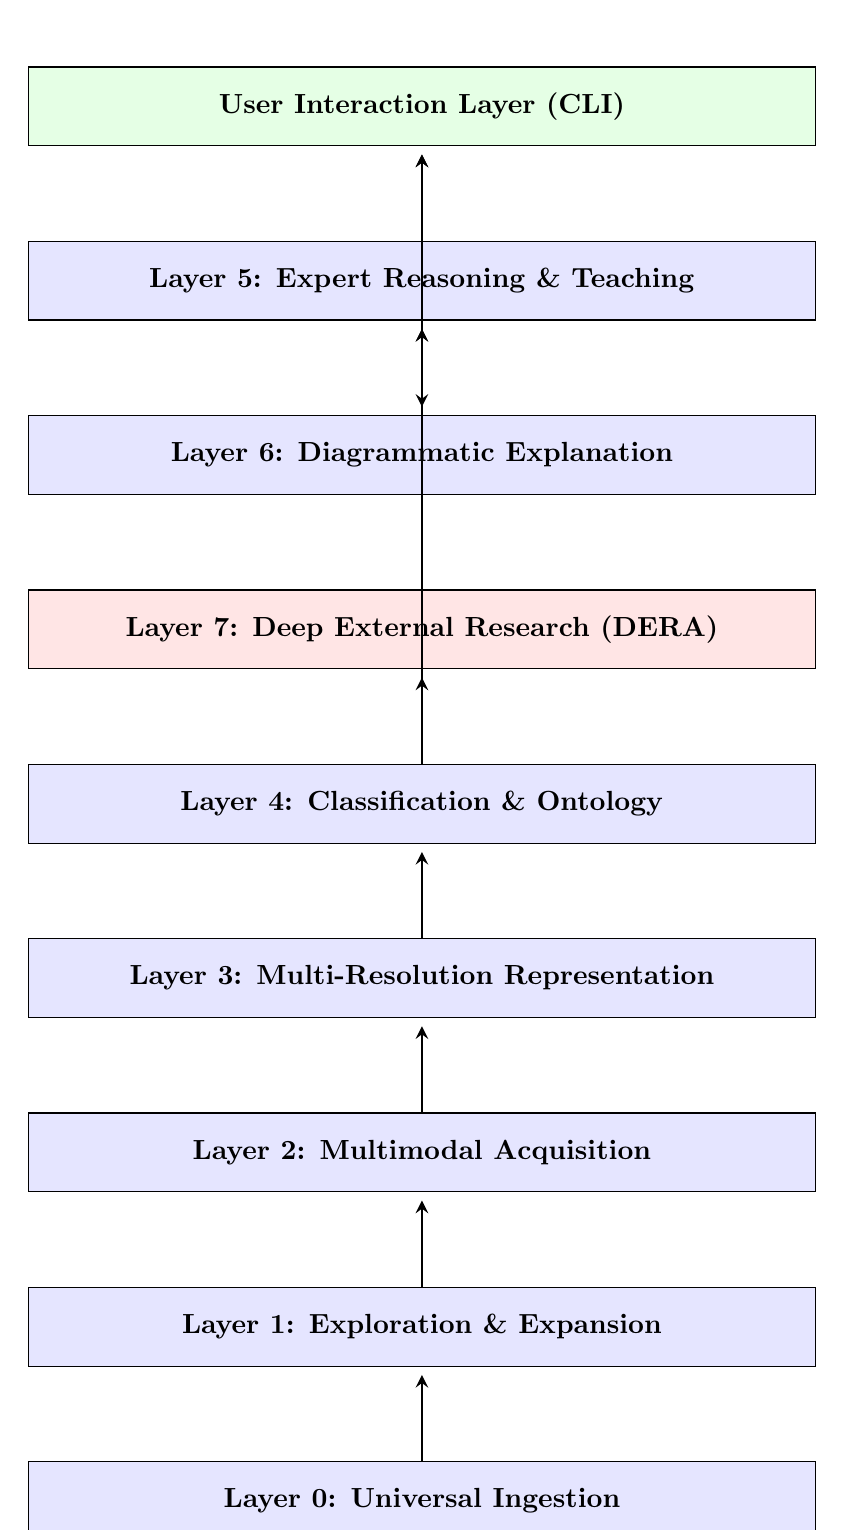
\begin{tikzpicture}[
    node distance=1.2cm,
    layer/.style={rectangle, draw, fill=blue!10, minimum width=10cm, minimum height=1cm, align=center},
    deep/.style={rectangle, draw, fill=red!10, minimum width=10cm, minimum height=1cm, align=center},
    interface/.style={rectangle, draw, fill=green!10, minimum width=10cm, minimum height=1cm, align=center},
    arrow/.style={->, >=stealth, line width=1pt, shorten >=3pt}
]

\node[interface] (ui) {\textbf{User Interaction Layer (CLI)}};
\node[layer, below=of ui] (l5) {\textbf{Layer 5: Expert Reasoning \& Teaching}};
\node[layer, below=of l5] (l6) {\textbf{Layer 6: Diagrammatic Explanation}};
\node[deep, below=of l6] (l7) {\textbf{Layer 7: Deep External Research (DERA)}};
\node[layer, below=of l7] (l4) {\textbf{Layer 4: Classification \& Ontology}};
\node[layer, below=of l4] (l3) {\textbf{Layer 3: Multi-Resolution Representation}};
\node[layer, below=of l3] (l2) {\textbf{Layer 2: Multimodal Acquisition}};
\node[layer, below=of l2] (l1) {\textbf{Layer 1: Exploration \& Expansion}};
\node[layer, below=of l1] (l0) {\textbf{Layer 0: Universal Ingestion}};

\draw[arrow] (l0) -- (l1);
\draw[arrow] (l1) -- (l2);
\draw[arrow] (l2) -- (l3);
\draw[arrow] (l3) -- (l4);
\draw[arrow] (l4) -- (l5);
\draw[arrow] (l5) -- (l6);
\draw[arrow] (l4) -- (l7);
\draw[arrow] (l7) -- (l5);
\draw[arrow] (l5) -- (ui);
\draw[arrow] (l6) -- (ui);

\end{tikzpicture}
\caption{KNOWY Layered Architecture with Shallow-Deep Agent Separation}
\label{fig:architecture}
\end{figure}

\subsection{Architectural Guarantees}

\begin{table}[H]
\centering
\begin{tabular}{@{}lp{10cm}@{}}
\toprule
\textbf{Guarantee} & \textbf{Implementation Mechanism} \\
\midrule
Epistemic Boundary Preservation & Type-level enforcement in orchestration graph; shallow agents cannot invoke external knowledge sources \\
\addlinespace
Hallucination Minimization & Multi-resolution grounding with explicit provenance tracking; uncertainty quantification at reasoning layer \\
\addlinespace
Temporal Consistency & Versioned knowledge representations with timestamp-based validity windows \\
\addlinespace
Multimodal Coherence & Unified semantic representation across text, video frames, and diagrams with cross-modal alignment \\
\addlinespace
Reproducibility & Deterministic agent execution with comprehensive logging; CLI-based workflow capture \\
\bottomrule
\end{tabular}
\caption{Core Architectural Guarantees}
\label{tab:guarantees}
\end{table}

\subsection{Technology Stack}

\begin{table}[H]
\centering
\begin{tabular}{@{}llp{6cm}@{}}
\toprule
\textbf{Component} & \textbf{Technology} & \textbf{Justification} \\
\midrule
Agent Orchestration & LangGraph & Graph-based execution with conditional routing and state management \\
\addlinespace
Local LLM Runtime & Ollama & Unified API for multiple local models; efficient inference \\
\addlinespace
Text Models & LLaMA 3.x, Qwen, Gemma & State-of-the-art reasoning with local deployment \\
\addlinespace
Multimodal Models & LLaMA 3.2 Vision & Native image understanding for video frame analysis \\
\addlinespace
Video Analysis & video-analyzer & Shot segmentation, transcript alignment, visual-semantic extraction \\
\addlinespace
CLI Framework & llm (Simon Willison) & Plugin architecture, scriptability, model abstraction \\
\addlinespace
Vector Database & FAISS / Qdrant & High-performance similarity search with filtering \\
\addlinespace
Structured Storage & PostgreSQL + Neo4j & Relational metadata + graph-based ontologies \\
\addlinespace
Diagram Generation & Graphviz, Mermaid & Programmatic schematic creation \\
\bottomrule
\end{tabular}
\caption{Technology Stack Components}
\label{tab:techstack}
\end{table}

\section{Layer 0: Universal Ingestion}

\subsection{Purpose and Epistemic Question}

\textbf{Epistemic Question}: \textit{"What reference has the user saved, independent of format or source?"}

Layer 0 establishes the entry point for all knowledge artifacts entering the system. It normalizes heterogeneous inputs from browsers, LinkedIn saves, manual entries, and API integrations into a canonical source descriptor format.

\subsection{Canonical Source Descriptor Schema}

\begin{lstlisting}[language=Python, caption=Canonical Source Descriptor Data Structure]
from dataclasses import dataclass
from typing import List, Optional, Dict
from datetime import datetime
from uuid import UUID

@dataclass
class ContentHints:
    contains_pdf: bool
    contains_video: bool
    contains_external_links: bool
    contains_code_repository: bool
    estimated_length_minutes: Optional[int]
    primary_language: Optional[str]

@dataclass
class CanonicalSourceDescriptor:
    source_id: UUID
    origin: str  # linkedin | browser | manual | api | other
    raw_reference: str
    raw_text: Optional[str]
    links: List[str]
    content_hints: ContentHints
    timestamp: datetime
    ingestion_metadata: Dict[str, any]
    
    def to_json(self) -> dict:
        """Serialize to storage format"""
        pass
    
    @classmethod
    def from_raw_input(cls, raw_input: str, origin: str):
        """Factory method for ingestion"""
        pass
\end{lstlisting}

\subsection{Ingestion Pipeline Architecture}

\begin{figure}[H]
\centering
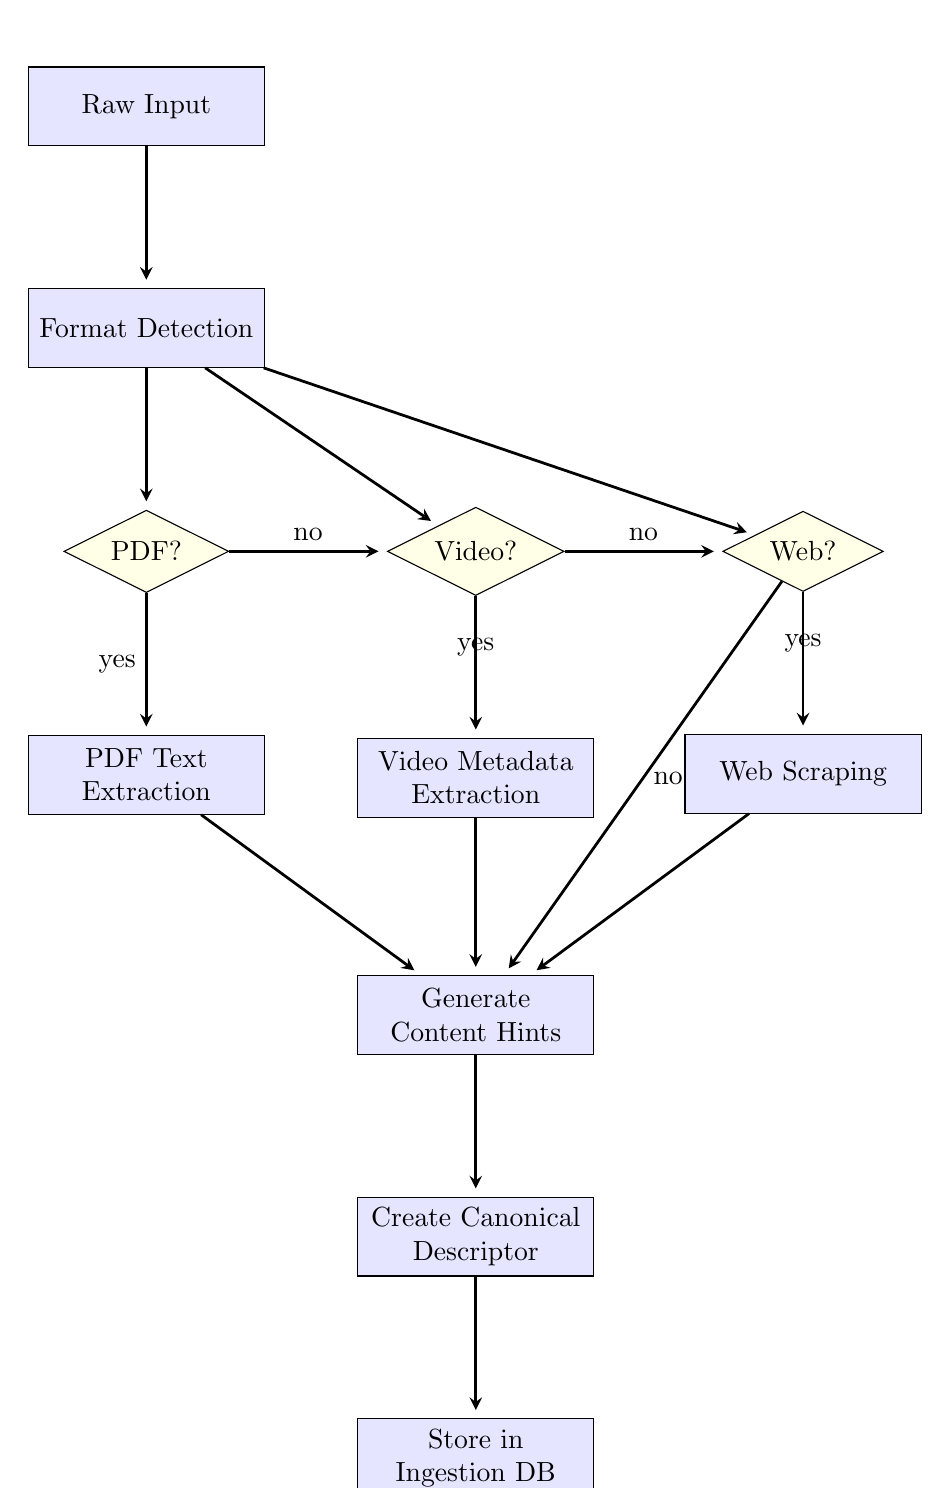
\begin{tikzpicture}[
    node distance=1.8cm,
    box/.style={rectangle, draw, fill=blue!10, minimum width=3cm, minimum height=1cm, align=center},
    decision/.style={diamond, draw, fill=yellow!10, aspect=2, align=center},
    arrow/.style={->, >=stealth, line width=1pt, shorten >=3pt}
]

\node[box] (input) {Raw Input};
\node[box, below=of input] (detect) {Format Detection};
\node[decision, below=of detect] (pdf) {PDF?};
\node[decision, right=2cm of pdf] (video) {Video?};
\node[decision, right=2cm of video] (web) {Web?};
\node[box, below=of pdf] (extract_pdf) {PDF Text\\Extraction};
\node[box, below=of video] (extract_video) {Video Metadata\\Extraction};
\node[box, below=of web] (extract_web) {Web Scraping};
\node[box, below=2cm of extract_video] (hints) {Generate\\Content Hints};
\node[box, below=of hints] (descriptor) {Create Canonical\\Descriptor};
\node[box, below=of descriptor] (store) {Store in\\Ingestion DB};

\draw[arrow] (input) -- (detect);
\draw[arrow] (detect) -- (pdf);
\draw[arrow] (pdf) -- node[left] {yes} (extract_pdf);
\draw[arrow] (detect) -- (video);
\draw[arrow] (video) -- node[above] {yes} (extract_video);
\draw[arrow] (detect) -- (web);
\draw[arrow] (web) -- node[above] {yes} (extract_web);
\draw[arrow] (extract_pdf) -- (hints);
\draw[arrow] (extract_video) -- (hints);
\draw[arrow] (extract_web) -- (hints);
\draw[arrow] (pdf) -- node[above] {no} (video);
\draw[arrow] (video) -- node[above] {no} (web);
\draw[arrow] (web) -- node[right] {no} (hints);
\draw[arrow] (hints) -- (descriptor);
\draw[arrow] (descriptor) -- (store);

\end{tikzpicture}
\caption{Layer 0 Ingestion Pipeline}
\label{fig:ingestion}
\end{figure}

\subsection{Browser Extension Integration}

\begin{lstlisting}[language=JavaScript, caption=Browser Extension Content Script]
// KNOWY Browser Extension - Content Script
class KnowyExtension {
  constructor(apiEndpoint) {
    this.apiEndpoint = apiEndpoint;
  }
  
  async captureCurrentPage() {
    const pageData = {
      url: window.location.href,
      title: document.title,
      selectedText: window.getSelection().toString(),
      fullText: document.body.innerText,
      links: Array.from(document.querySelectorAll('a'))
        .map(a => a.href),
      timestamp: new Date().toISOString()
    };
    
    return await this.sendToKnowy(pageData);
  }
  
  async sendToKnowy(data) {
    const response = await fetch(`${this.apiEndpoint}/ingest`, {
      method: 'POST',
      headers: {'Content-Type': 'application/json'},
      body: JSON.stringify({
        origin: 'browser',
        raw_reference: data.url,
        raw_text: data.fullText,
        links: data.links,
        metadata: {title: data.title, selectedText: data.selectedText}
      })
    });
    return response.json();
  }
}
\end{lstlisting}

\subsection{Format Detection Algorithm}

\begin{algorithm}[H]
\caption{Format Detection and Content Hint Generation}
\begin{algorithmic}[1]
\REQUIRE Raw input string $I$, origin metadata $O$
\ENSURE ContentHints object $H$
\STATE $H \gets \text{new ContentHints()}$
\IF{$I$ matches URL pattern}
    \STATE $domain \gets \text{extractDomain}(I)$
    \IF{$domain \in \{\text{youtube.com}, \text{vimeo.com}, \text{coursera.org}\}$}
        \STATE $H.\text{contains\_video} \gets \text{true}$
        \STATE $H.\text{estimated\_length\_minutes} \gets \text{estimateFromMetadata}(I)$
    \ELSIF{$domain$ ends with .pdf}
        \STATE $H.\text{contains\_pdf} \gets \text{true}$
    \ELSE
        \STATE $content \gets \text{fetchHTMLHead}(I)$
        \STATE $H \gets \text{analyzeOpenGraph}(content)$
    \ENDIF
\ELSIF{$I$ matches file path pattern}
    \STATE $extension \gets \text{getExtension}(I)$
    \STATE $H \gets \text{mapExtensionToHints}(extension)$
\ELSE
    \STATE $H.\text{contains\_external\_links} \gets \text{detectURLs}(I)$
\ENDIF
\RETURN $H$
\end{algorithmic}
\end{algorithm}

\subsection{Storage Schema}

\begin{lstlisting}[language=SQL, caption=Ingestion Database Schema]
CREATE TABLE ingestion_sources (
    source_id UUID PRIMARY KEY,
    origin VARCHAR(50) NOT NULL,
    raw_reference TEXT NOT NULL,
    raw_text TEXT,
    links JSONB,
    content_hints JSONB NOT NULL,
    timestamp TIMESTAMPTZ NOT NULL,
    ingestion_metadata JSONB,
    processing_status VARCHAR(20) DEFAULT 'pending',
    created_at TIMESTAMPTZ DEFAULT NOW()
);

CREATE INDEX idx_origin ON ingestion_sources(origin);
CREATE INDEX idx_timestamp ON ingestion_sources(timestamp);
CREATE INDEX idx_status ON ingestion_sources(processing_status);
CREATE INDEX idx_hints_gin ON ingestion_sources USING GIN(content_hints);
\end{lstlisting}

\section{Layer 1: Exploration and Expansion}

\subsection{Purpose and Epistemic Question}

\textbf{Epistemic Question}: \textit{"What actual knowledge artifacts exist behind this reference?"}

Layer 1 performs deep link analysis and reference expansion. A single user-saved URL may reference multiple papers, course modules, or video playlists that constitute distinct knowledge artifacts requiring separate processing.

\subsection{Expansion Agent Architecture}

\begin{lstlisting}[language=Python, caption=Exploration Agent Implementation]
from typing import List, Set
from langchain.agents import AgentExecutor
from langchain.tools import Tool

class ExplorationAgent:
    def __init__(self, llm, web_browser_tool):
        self.llm = llm
        self.browser = web_browser_tool
        self.discovered_artifacts = []
        
    async def expand_reference(self, 
                               source_descriptor: CanonicalSourceDescriptor
                              ) -> List[KnowledgeArtifact]:
        """
        Expand a source descriptor into constituent knowledge artifacts.
        """
        artifacts = []
        
        # Analyze content hints to determine expansion strategy
        if source_descriptor.content_hints.contains_video:
            artifacts.extend(
                await self._expand_video_playlist(source_descriptor)
            )
        
        if source_descriptor.content_hints.contains_pdf:
            artifacts.extend(
                await self._expand_pdf_citations(source_descriptor)
            )
        
        if source_descriptor.content_hints.contains_external_links:
            artifacts.extend(
                await self._expand_linked_resources(source_descriptor)
            )
        
        # Use LLM to identify implicit references
        implicit_refs = await self._identify_implicit_references(
            source_descriptor.raw_text
        )
        artifacts.extend(implicit_refs)
        
        return self._deduplicate(artifacts)
    
    async def _expand_video_playlist(self, 
                                     source: CanonicalSourceDescriptor
                                    ) -> List[KnowledgeArtifact]:
        """Extract individual videos from playlists or courses."""
        # Implementation uses platform-specific APIs
        pass
    
    async def _expand_pdf_citations(self,
                                     source: CanonicalSourceDescriptor
                                    ) -> List[KnowledgeArtifact]:
        """Extract and resolve cited papers."""
        # Parse bibliography, resolve DOIs
        pass
    
    async def _identify_implicit_references(self, 
                                            text: str
                                           ) -> List[KnowledgeArtifact]:
        """Use LLM to identify mentioned resources."""
        prompt = f"""
        Analyze the following text and identify any academic papers,
        books, courses, or other knowledge resources that are mentioned
        but not explicitly linked. For each, provide:
        - Resource type (paper/book/course/video)
        - Title
        - Author(s) if mentioned
        - Any identifying information (DOI, ISBN, URL)
        
        Text: {text}
        
        Return as structured JSON.
        """
        response = await self.llm.ainvoke(prompt)
        return self._parse_artifact_json(response)
\end{lstlisting}

\subsection{Knowledge Artifact Data Structure}

\begin{lstlisting}[language=Python, caption=Knowledge Artifact Schema]
from enum import Enum

class ArtifactType(Enum):
    PAPER = "academic_paper"
    BOOK = "book"
    COURSE = "online_course"
    VIDEO_LECTURE = "video_lecture"
    BLOG_POST = "blog_post"
    DOCUMENTATION = "technical_documentation"
    DATASET = "dataset"
    CODE_REPOSITORY = "code_repository"

@dataclass
class KnowledgeArtifact:
    artifact_id: UUID
    source_id: UUID  # Links back to ingestion source
    artifact_type: ArtifactType
    title: str
    authors: List[str]
    url: Optional[str]
    doi: Optional[str]
    isbn: Optional[str]
    abstract: Optional[str]
    publication_date: Optional[datetime]
    acquisition_strategy: str  # Determines Layer 2 pipeline
    metadata: Dict[str, any]
    
    def requires_video_analysis(self) -> bool:
        return self.artifact_type in [
            ArtifactType.VIDEO_LECTURE,
            ArtifactType.COURSE
        ]
    
    def requires_pdf_processing(self) -> bool:
        return self.artifact_type in [
            ArtifactType.PAPER,
            ArtifactType.BOOK
        ] or (self.url and self.url.endswith('.pdf'))
\end{lstlisting}

\subsection{Reference Resolution Strategies}

\begin{table}[H]
\centering
\begin{tabular}{@{}lp{5cm}p{5cm}@{}}
\toprule
\textbf{Reference Type} & \textbf{Resolution Strategy} & \textbf{Tools/APIs} \\
\midrule
DOI & Query CrossRef API & \texttt{requests}, CrossRef REST API \\
\addlinespace
arXiv ID & Parse arXiv metadata & arXiv API \\
\addlinespace
ISBN & Query OpenLibrary & OpenLibrary API \\
\addlinespace
YouTube URL & Extract video/playlist ID & YouTube Data API \\
\addlinespace
Course Platform & Platform-specific scraping & Selenium, BeautifulSoup \\
\addlinespace
GitHub Repository & Clone and analyze structure & PyGithub, git \\
\addlinespace
Generic Web Page & Content extraction & Trafilatura, newspaper3k \\
\bottomrule
\end{tabular}
\caption{Reference Resolution Strategies by Type}
\label{tab:resolution}
\end{table}

\subsection{Deduplication Algorithm}

\begin{algorithm}[H]
\caption{Knowledge Artifact Deduplication}
\begin{algorithmic}[1]
\REQUIRE Set of artifacts $A = \{a_1, a_2, \ldots, a_n\}$
\ENSURE Deduplicated set $A'$
\STATE $A' \gets \emptyset$
\STATE $seen \gets \emptyset$
\FOR{$a \in A$}
    \STATE $key \gets \text{generateKey}(a)$
    \IF{$key \notin seen$}
        \STATE $A' \gets A' \cup \{a\}$
        \STATE $seen \gets seen \cup \{key\}$
    \ELSE
        \STATE $existing \gets \text{findByKey}(A', key)$
        \STATE $merged \gets \text{mergeMetadata}(existing, a)$
        \STATE \text{replace}$(existing, merged)$
    \ENDIF
\ENDFOR
\RETURN $A'$
\end{algorithmic}
\end{algorithm}

Where the key generation function prioritizes unique identifiers:
\begin{lstlisting}[language=Python, caption=Artifact Key Generation]
def generate_key(artifact: KnowledgeArtifact) -> str:
    if artifact.doi:
        return f"doi:{artifact.doi}"
    elif artifact.isbn:
        return f"isbn:{artifact.isbn}"
    elif artifact.url:
        return f"url:{normalize_url(artifact.url)}"
    else:
        # Fallback to content-based hash
        return f"hash:{hash_content(artifact.title, artifact.authors)}"
\end{lstlisting}

\section{Layer 2: Multimodal Acquisition and Scraping}

\subsection{Purpose and Epistemic Question}

\textbf{Epistemic Question}: \textit{"What is the complete primary content of each identified artifact?"}

Layer 2 implements specialized acquisition pipelines for different modalities and formats. The most sophisticated component is the video analysis pipeline, which transforms long-form lectures into structured knowledge units.

\subsection{Acquisition Pipeline Dispatcher}

\begin{lstlisting}[language=Python, caption=Acquisition Pipeline Orchestration]
class AcquisitionOrchestrator:
    def __init__(self):
        self.pipelines = {
            'pdf': PDFAcquisitionPipeline(),
            'video': VideoAnalysisPipeline(),
            'web': WebScrapingPipeline(),
            'code': CodeRepositoryPipeline(),
            'paper': AcademicPaperPipeline()
        }
    
    async def acquire(self, 
                      artifact: KnowledgeArtifact
                     ) -> AcquiredContent:
        pipeline = self._select_pipeline(artifact)
        
        try:
            content = await pipeline.acquire(artifact)
            validation_result = await self._validate_content(content)
            
            if validation_result.is_valid:
                return content
            else:
                # Attempt fallback pipeline
                fallback = self._get_fallback_pipeline(artifact)
                return await fallback.acquire(artifact)
                
        except AcquisitionException as e:
            # Log failure and return partial content
            self._log_acquisition_failure(artifact, e)
            return self._create_partial_content(artifact, e)
    
    def _select_pipeline(self, 
                        artifact: KnowledgeArtifact
                       ) -> AcquisitionPipeline:
        if artifact.requires_video_analysis():
            return self.pipelines['video']
        elif artifact.requires_pdf_processing():
            if artifact.doi or artifact.artifact_type == ArtifactType.PAPER:
                return self.pipelines['paper']
            else:
                return self.pipelines['pdf']
        elif artifact.artifact_type == ArtifactType.CODE_REPOSITORY:
            return self.pipelines['code']
        else:
            return self.pipelines['web']
\end{lstlisting}

\subsection{Video Analysis Pipeline Integration}

The video analysis pipeline integrates the open-source \texttt{video-analyzer} project to perform shot-level semantic extraction.

\subsubsection{Video Analysis Architecture}

\begin{figure}[H]
\centering
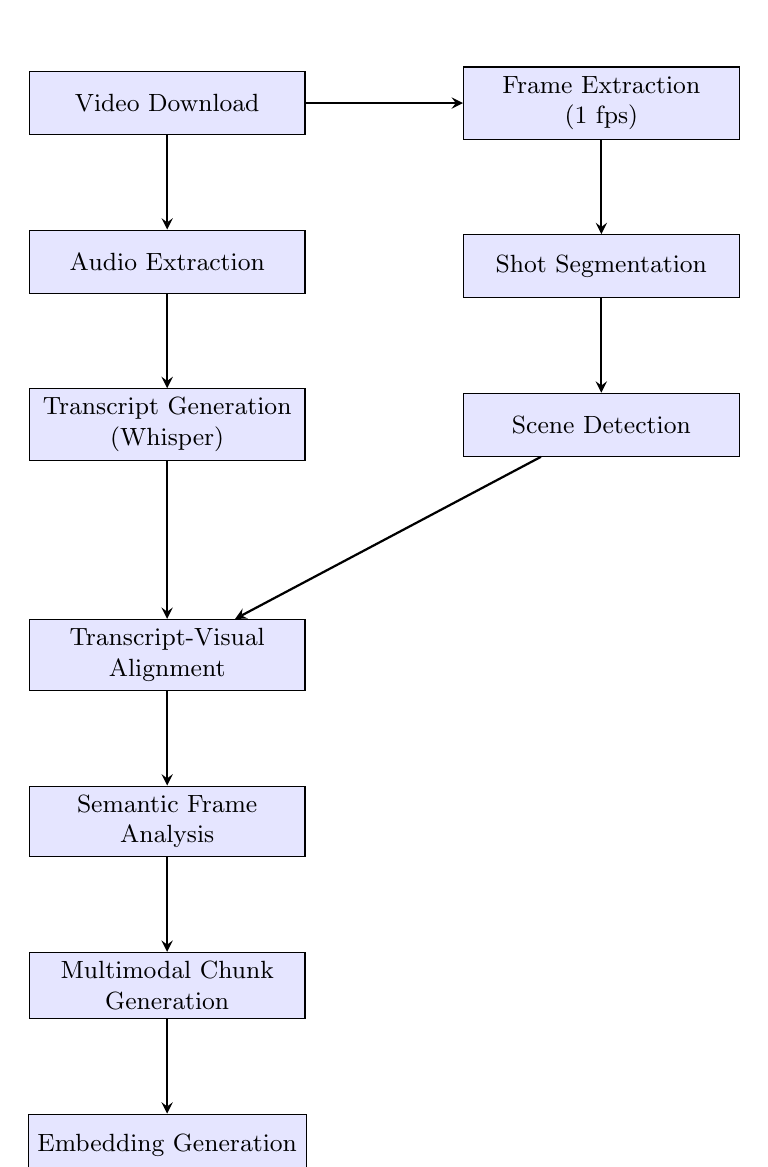
\begin{tikzpicture}[
    node distance=1.2cm,
    box/.style={rectangle, draw, fill=blue!10, minimum width=3.5cm, minimum height=0.8cm, align=center, font=\small},
    arrow/.style={->, >=stealth, thick}
]

\node[box] (download) {Video Download};
\node[box, below=of download] (audio) {Audio Extraction};
\node[box, below=of audio] (transcript) {Transcript Generation\\(Whisper)};
\node[box, right=2cm of download] (frame) {Frame Extraction\\(1 fps)};
\node[box, below=of frame] (shot) {Shot Segmentation};
\node[box, below=of shot] (scene) {Scene Detection};
\node[box, below=2cm of transcript] (align) {Transcript-Visual\\Alignment};
\node[box, below=of align] (semantic) {Semantic Frame\\Analysis};
\node[box, below=of semantic] (chunk) {Multimodal Chunk\\Generation};
\node[box, below=of chunk] (embed) {Embedding Generation};

\draw[arrow] (download) -- (audio);
\draw[arrow] (audio) -- (transcript);
\draw[arrow] (download) -- (frame);
\draw[arrow] (frame) -- (shot);
\draw[arrow] (shot) -- (scene);
\draw[arrow] (transcript) -- (align);
\draw[arrow] (scene) -- (align);
\draw[arrow] (align) -- (semantic);
\draw[arrow] (semantic) -- (chunk);
\draw[arrow] (chunk) -- (embed);

\end{tikzpicture}
\caption{Video Analysis Pipeline Architecture}
\label{fig:video_pipeline}
\end{figure}

\subsubsection{Shot Segmentation Algorithm}

\begin{algorithm}[H]
\caption{Adaptive Shot Boundary Detection}
\begin{algorithmic}[1]
\REQUIRE Video frames $F = \{f_1, f_2, \ldots, f_n\}$, threshold $\tau$
\ENSURE Shot boundaries $B = \{b_1, b_2, \ldots, b_m\}$
\STATE $B \gets \emptyset$
\STATE $prev\_hist \gets \text{computeHistogram}(f_1)$
\FOR{$i \gets 2$ to $n$}
    \STATE $curr\_hist \gets \text{computeHistogram}(f_i)$
    \STATE $diff \gets \text{histogramDistance}(prev\_hist, curr\_hist)$
    \IF{$diff > \tau$}
        \STATE $B \gets B \cup \{i\}$
        \STATE $\tau \gets \text{adaptThreshold}(\tau, diff)$
    \ENDIF
    \STATE $prev\_hist \gets curr\_hist$
\ENDFOR
\RETURN $B$
\end{algorithmic}
\end{algorithm}

\subsubsection{Transcript-Visual Alignment}

\begin{lstlisting}[language=Python, caption=Transcript-Visual Temporal Alignment]
class TranscriptVisualAligner:
    def __init__(self, whisper_model):
        self.whisper = whisper_model
        
    async def align(self, 
                    transcript_segments: List[TranscriptSegment],
                    shots: List[Shot]) -> List[AlignedChunk]:
        """
        Align transcript segments with visual shots to create
        semantically coherent multimodal chunks.
        """
        aligned_chunks = []
        shot_idx = 0
        
        for segment in transcript_segments:
            # Find overlapping shots
            overlapping_shots = []
            while (shot_idx < len(shots) and 
                   shots[shot_idx].start_time <= segment.end_time):
                if shots[shot_idx].end_time >= segment.start_time:
                    overlapping_shots.append(shots[shot_idx])
                shot_idx += 1
            
            # Create aligned chunk
            chunk = AlignedChunk(
                start_time=segment.start_time,
                end_time=segment.end_time,
                transcript_text=segment.text,
                shots=overlapping_shots,
                speaker=segment.speaker,
                confidence=segment.confidence
            )
            
            aligned_chunks.append(chunk)
        
        return aligned_chunks

@dataclass
class AlignedChunk:
    start_time: float
    end_time: float
    transcript_text: str
    shots: List[Shot]
    speaker: Optional[str]
    confidence: float
    
    def get_representative_frame(self) -> np.ndarray:
        """Select most informative frame from shots."""
        if not self.shots:
            return None
        # Use middle frame of longest shot
        longest_shot = max(self.shots, key=lambda s: s.duration)
        return longest_shot.frames[len(longest_shot.frames) // 2]
\end{lstlisting}

\subsubsection{Semantic Frame Analysis}

\begin{lstlisting}[language=Python, caption=Visual-Semantic Frame Analysis with LLaMA Vision]
class SemanticFrameAnalyzer:
    def __init__(self, vision_model):
        self.vision_model = vision_model  # LLaMA 3.2 Vision
        
    async def analyze_chunk(self, 
                           chunk: AlignedChunk
                          ) -> SemanticAnalysis:
        """
        Perform semantic analysis of visual content in context
        of transcript.
        """
        frame = chunk.get_representative_frame()
        
        prompt = f"""
        Analyze this frame from an educational video lecture.
        
        Transcript context: "{chunk.transcript_text}"
        
        Describe:
        1. Visual content (diagrams, equations, code, slides)
        2. Key concepts being illustrated
        3. Relationship between visual and spoken content
        4. Educational value of this visual
        
        Provide structured analysis.
        """
        
        analysis = await self.vision_model.analyze(
            image=frame,
            prompt=prompt
        )
        
        return SemanticAnalysis(
            chunk_id=chunk.id,
            visual_description=analysis.visual_content,
            concepts=analysis.key_concepts,
            visual_transcript_coherence=analysis.coherence_score,
            educational_value=analysis.educational_value,
            contains_diagram=self._detect_diagram(analysis),
            contains_equation=self._detect_equation(analysis),
            contains_code=self._detect_code(analysis)
        )
\end{lstlisting}

\subsubsection{Multimodal Chunk Generation}

\begin{lstlisting}[language=Python, caption=Complete Multimodal Chunk Data Structure]
@dataclass
class MultimodalChunk:
    chunk_id: UUID
    artifact_id: UUID
    temporal_range: Tuple[float, float]
    
    # Textual components
    transcript_text: str
    transcript_confidence: float
    
    # Visual components
    representative_frame: bytes  # JPEG-encoded
    all_frames: List[bytes]
    shot_boundaries: List[float]
    
    # Semantic analysis
    visual_description: str
    key_concepts: List[str]
    contains_diagram: bool
    contains_equation: bool
    contains_code: bool
    
    # Embeddings
    text_embedding: np.ndarray
    visual_embedding: np.ndarray
    combined_embedding: np.ndarray
    
    # Metadata
    speaker: Optional[str]
    slide_number: Optional[int]
    topic_tags: List[str]
    
    def to_storage_format(self) -> dict:
        """Prepare for database insertion."""
        return {
            'chunk_id': str(self.chunk_id),
            'artifact_id': str(self.artifact_id),
            'temporal_range': self.temporal_range,
            'transcript_text': self.transcript_text,
            'visual_description': self.visual_description,
            'key_concepts': json.dumps(self.key_concepts),
            'semantic_flags': {
                'diagram': self.contains_diagram,
                'equation': self.contains_equation,
                'code': self.contains_code
            },
            'embeddings': {
                'text': self.text_embedding.tolist(),
                'visual': self.visual_embedding.tolist(),
                'combined': self.combined_embedding.tolist()
            }
        }
\end{lstlisting}

\subsection{PDF Acquisition Pipeline}

\begin{lstlisting}[language=Python, caption=PDF Processing with Layout Preservation]
class PDFAcquisitionPipeline:
    def __init__(self):
        self.extractors = {
            'text': PDFTextExtractor(),
            'layout': PDFLayoutExtractor(),
            'images': PDFImageExtractor(),
            'tables': PDFTableExtractor()
        }
    
    async def acquire(self, artifact: KnowledgeArtifact) -> PDFContent:
        pdf_bytes = await self._download_pdf(artifact.url)
        
        # Parallel extraction
        text_task = self.extractors['text'].extract(pdf_bytes)
        layout_task = self.extractors['layout'].extract(pdf_bytes)
        images_task = self.extractors['images'].extract(pdf_bytes)
        tables_task = self.extractors['tables'].extract(pdf_bytes)
        
        text, layout, images, tables = await asyncio.gather(
            text_task, layout_task, images_task, tables_task
        )
        
        # Reconstruct document structure
        structured_content = self._reconstruct_structure(
            text, layout, images, tables
        )
        
        return PDFContent(
            artifact_id=artifact.artifact_id,
            raw_text=text.full_text,
            sections=structured_content.sections,
            figures=images,
            tables=tables,
            citations=self._extract_citations(text),
            metadata=self._extract_metadata(pdf_bytes)
        )
    
    def _reconstruct_structure(self, text, layout, images, tables):
        """
        Reconstruct document hierarchy using layout analysis.
        Preserves section headers, paragraphs, lists, etc.
        """
        sections = []
        current_section = None
        
        for block in layout.blocks:
            if block.type == 'heading':
                if current_section:
                    sections.append(current_section)
                current_section = Section(
                    title=block.text,
                    level=block.heading_level,
                    content=[]
                )
            elif block.type == 'paragraph':
                if current_section:
                    current_section.content.append(
                        Paragraph(text=block.text)
                    )
            elif block.type == 'figure':
                fig = self._match_figure(block, images)
                if current_section and fig:
                    current_section.content.append(fig)
            elif block.type == 'table':
                tbl = self._match_table(block, tables)
                if current_section and tbl:
                    current_section.content.append(tbl)
        
        if current_section:
            sections.append(current_section)
        
        return StructuredDocument(sections=sections)
\end{lstlisting}

\subsection{Academic Paper Pipeline}

\begin{lstlisting}[language=Python, caption=Academic Paper Specialized Processing]
class AcademicPaperPipeline:
    def __init__(self):
        self.pdf_pipeline = PDFAcquisitionPipeline()
        self.metadata_enricher = PaperMetadataEnricher()
        
    async def acquire(self, artifact: KnowledgeArtifact) -> PaperContent:
        # First get PDF content
        pdf_content = await self.pdf_pipeline.acquire(artifact)
        
        # Enrich with academic metadata
        metadata = await self.metadata_enricher.enrich(
            doi=artifact.doi,
            arxiv_id=self._extract_arxiv_id(artifact.url)
        )
        
        # Parse academic structure
        academic_structure = self._parse_academic_structure(
            pdf_content
        )
        
        return PaperContent(
            artifact_id=artifact.artifact_id,
            title=metadata.title or artifact.title,
            authors=metadata.authors or artifact.authors,
            abstract=academic_structure.abstract,
            introduction=academic_structure.introduction,
            methodology=academic_structure.methodology,
            results=academic_structure.results,
            discussion=academic_structure.discussion,
            conclusion=academic_structure.conclusion,
            references=pdf_content.citations,
            figures=pdf_content.figures,
            tables=pdf_content.tables,
            equations=self._extract_equations(pdf_content),
            citation_count=metadata.citation_count,
            publication_venue=metadata.venue,
            publication_date=metadata.publication_date
        )
    
    def _parse_academic_structure(self, pdf_content):
        """
        Use section headers to identify standard paper sections.
        """
        section_map = {
            'abstract': None,
            'introduction': None,
            'methodology': None,
            'results': None,
            'discussion': None,
            'conclusion': None
        }
        
        for section in pdf_content.sections:
            title_lower = section.title.lower()
            
            if 'abstract' in title_lower:
                section_map['abstract'] = section
            elif 'introduction' in title_lower:
                section_map['introduction'] = section
            elif any(kw in title_lower for kw in 
                    ['method', 'approach', 'design']):
                section_map['methodology'] = section
            elif 'result' in title_lower:
                section_map['results'] = section
            elif 'discussion' in title_lower:
                section_map['discussion'] = section
            elif 'conclusion' in title_lower:
                section_map['conclusion'] = section
        
        return AcademicStructure(**section_map)
\end{lstlisting}

\section{Layer 3: Multi-Resolution Knowledge Representation}

\subsection{Purpose and Epistemic Question}

\textbf{Epistemic Question}: \textit{"How should knowledge be structured at multiple levels of abstraction to support both factual grounding and high-level reasoning?"}

Layer 3 constructs a four-level abstraction hierarchy that enables both precise fact retrieval and synthesized understanding.

\subsection{Four-Level Abstraction Hierarchy}

\begin{table}[H]
\centering
\begin{tabular}{@{}lp{5cm}p{5cm}@{}}
\toprule
\textbf{Level} & \textbf{Granularity} & \textbf{Use Case} \\
\midrule
Level 0 & Raw chunks (paragraphs, video segments) & Direct citation, fact verification \\
\addlinespace
Level 1 & Section-level summaries & Navigating document structure \\
\addlinespace
Level 2 & Document-level synthesis & Comparing papers, course overview \\
\addlinespace
Level 3 & Cross-document thematic synthesis & Domain understanding, research frontiers \\
\bottomrule
\end{tabular}
\caption{Multi-Resolution Abstraction Levels}
\label{tab:abstraction}
\end{table}

\subsection{Representation Architecture}

\begin{figure}[H]
\centering
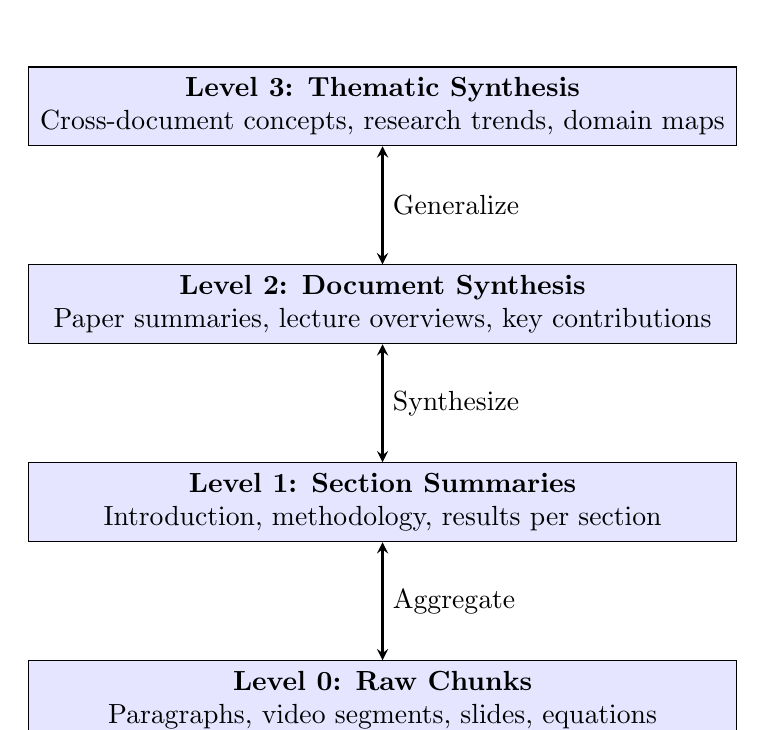
\begin{tikzpicture}[
    node distance=1.5cm,
    level/.style={rectangle, draw, fill=blue!10, minimum width=9cm, minimum height=1cm, align=center},
    arrow/.style={<->, >=stealth, thick}
]

\node[level] (l3) {\textbf{Level 3: Thematic Synthesis}\\Cross-document concepts, research trends, domain maps};
\node[level, below=of l3] (l2) {\textbf{Level 2: Document Synthesis}\\Paper summaries, lecture overviews, key contributions};
\node[level, below=of l2] (l1) {\textbf{Level 1: Section Summaries}\\Introduction, methodology, results per section};
\node[level, below=of l1] (l0) {\textbf{Level 0: Raw Chunks}\\Paragraphs, video segments, slides, equations};

\draw[arrow] (l0) -- node[right] {Aggregate} (l1);
\draw[arrow] (l1) -- node[right] {Synthesize} (l2);
\draw[arrow] (l2) -- node[right] {Generalize} (l3);

\end{tikzpicture}
\caption{Multi-Resolution Representation Hierarchy}
\label{fig:multiresolution}
\end{figure}

\subsection{Level 0: Raw Content Storage}

\begin{lstlisting}[language=Python, caption=Level 0 Raw Chunk Representation]
@dataclass
class RawChunk:
    chunk_id: UUID
    artifact_id: UUID
    chunk_type: str  # paragraph | video_segment | equation | figure
    
    # Content
    text_content: Optional[str]
    visual_content: Optional[bytes]
    structured_content: Optional[dict]  # For tables, code
    
    # Positional metadata
    position_in_artifact: int
    section_id: Optional[UUID]
    temporal_range: Optional[Tuple[float, float]]  # For video
    page_number: Optional[int]  # For PDFs
    
    # Embeddings
    embedding: np.ndarray
    
    # Provenance
    extraction_method: str
    confidence: float
    
    def get_context_window(self, 
                          window_size: int = 2
                         ) -> List['RawChunk']:
        """Retrieve neighboring chunks for context."""
        pass

# Storage schema
CREATE TABLE raw_chunks (
    chunk_id UUID PRIMARY KEY,
    artifact_id UUID REFERENCES knowledge_artifacts(artifact_id),
    chunk_type VARCHAR(50),
    text_content TEXT,
    visual_content BYTEA,
    structured_content JSONB,
    position_in_artifact INTEGER,
    section_id UUID,
    temporal_range NUMRANGE,
    page_number INTEGER,
    embedding vector(1536),
    extraction_metadata JSONB,
    created_at TIMESTAMPTZ DEFAULT NOW()
);

CREATE INDEX idx_artifact ON raw_chunks(artifact_id);
CREATE INDEX idx_section ON raw_chunks(section_id);
CREATE INDEX idx_embedding ON raw_chunks 
    USING ivfflat (embedding vector_cosine_ops);
\end{lstlisting}

\subsection{Level 1: Section-Level Representation}

\begin{lstlisting}[language=Python, caption=Level 1 Section Summary Generation]
class SectionSummarizer:
    def __init__(self, llm):
        self.llm = llm
        
    async def generate_section_summary(self,
                                       section_chunks: List[RawChunk]
                                      ) -> SectionRepresentation:
        """
        Generate structured summary of a document section.
        """
        # Concatenate section content
        full_text = "
".join([
            chunk.text_content for chunk in section_chunks
            if chunk.text_content
        ])
        
        prompt = f"""
        Summarize the following section from an academic document.
        Provide:
        1. Main claim or thesis (1-2 sentences)
        2. Key points (bullet list)
        3. Important terminology defined
        4. Figures/equations referenced
        5. Dependencies on other sections
        
        Section content:
        {full_text}
        
        Output as structured JSON.
        """
        
        summary = await self.llm.ainvoke(prompt)
        parsed = json.loads(summary)
        
        return SectionRepresentation(
            section_id=uuid4(),
            artifact_id=section_chunks[0].artifact_id,
            title=self._extract_section_title(section_chunks),
            main_claim=parsed['main_claim'],
            key_points=parsed['key_points'],
            terminology=parsed['terminology'],
            referenced_elements=parsed['references'],
            chunk_ids=[c.chunk_id for c in section_chunks],
            embedding=await self._embed_summary(parsed['main_claim'])
        )

@dataclass
class SectionRepresentation:
    section_id: UUID
    artifact_id: UUID
    title: str
    main_claim: str
    key_points: List[str]
    terminology: Dict[str, str]
    referenced_elements: List[str]
    chunk_ids: List[UUID]
    embedding: np.ndarray
    prerequisites: List[UUID] = field(default_factory=list)
\end{lstlisting}

\subsection{Level 2: Document-Level Synthesis}

\begin{lstlisting}[language=Python, caption=Level 2 Document Synthesis]
class DocumentSynthesizer:
    def __init__(self, llm):
        self.llm = llm
        
    async def synthesize_document(self,
                                  sections: List[SectionRepresentation]
                                 ) -> DocumentRepresentation:
        """
        Create document-level synthesis from section summaries.
        """
        # Construct synthesis prompt
        section_summaries = "
".join([
            f"Section: {s.title}
Main claim: {s.main_claim}
"
            for s in sections
        ])
        
        prompt = f"""
        Synthesize the following academic document into a cohesive summary.
        
        Sections:
        {section_summaries}
        
        Provide:
        1. Central thesis (2-3 sentences)
        2. Main contributions (numbered list)
        3. Methodology overview
        4. Key findings
        5. Limitations discussed
        6. Related work positioning
        7. Novel concepts introduced
        
        Output as structured JSON.
        """
        
        synthesis = await self.llm.ainvoke(prompt)
        parsed = json.loads(synthesis)
        
        return DocumentRepresentation(
            document_id=uuid4(),
            artifact_id=sections[0].artifact_id,
            central_thesis=parsed['central_thesis'],
            contributions=parsed['contributions'],
            methodology=parsed['methodology'],
            findings=parsed['findings'],
            limitations=parsed['limitations'],
            novel_concepts=parsed['novel_concepts'],
            section_ids=[s.section_id for s in sections],
            embedding=await self._embed_synthesis(
                parsed['central_thesis']
            )
        )

@dataclass
class DocumentRepresentation:
    document_id: UUID
    artifact_id: UUID
    central_thesis: str
    contributions: List[str]
    methodology: str
    findings: List[str]
    limitations: List[str]
    novel_concepts: List[str]
    section_ids: List[UUID]
    embedding: np.ndarray
    citation_graph: Optional[dict] = None
\end{lstlisting}

\subsection{Level 3: Cross-Document Thematic Synthesis}

\begin{lstlisting}[language=Python, caption=Level 3 Thematic Synthesis]
class ThematicSynthesizer:
    def __init__(self, llm, clustering_model):
        self.llm = llm
        self.clusterer = clustering_model
        
    async def synthesize_themes(self,
                                documents: List[DocumentRepresentation]
                               ) -> List[ThematicSynthesis]:
        """
        Identify cross-document themes and research trends.
        """
        # Cluster documents by embedding similarity
        embeddings = np.array([d.embedding for d in documents])
        clusters = self.clusterer.fit_predict(embeddings)
        
        themes = []
        for cluster_id in np.unique(clusters):
            cluster_docs = [
                documents[i] for i in range(len(documents))
                if clusters[i] == cluster_id
            ]
            
            theme = await self._synthesize_cluster(cluster_docs)
            themes.append(theme)
        
        return themes
    
    async def _synthesize_cluster(self,
                                  docs: List[DocumentRepresentation]
                                 ) -> ThematicSynthesis:
        """
        Synthesize a thematic cluster into unified understanding.
        """
        # Extract key concepts across documents
        all_concepts = []
        all_theses = []
        
        for doc in docs:
            all_concepts.extend(doc.novel_concepts)
            all_theses.append(doc.central_thesis)
        
        prompt = f"""
        Analyze the following related research documents and identify:
        
        1. Common theme or research question
        2. Points of agreement
        3. Points of disagreement/debate
        4. Evolution of ideas (temporal if dates available)
        5. Open questions in this area
        6. Key terminology and definitions
        
        Document theses:
        {chr(10).join([f"- {t}" for t in all_theses])}
        
        Novel concepts mentioned:
        {chr(10).join([f"- {c}" for c in set(all_concepts)])}
        
        Output as structured JSON.
        """
        
        synthesis = await self.llm.ainvoke(prompt)
        parsed = json.loads(synthesis)
        
        return ThematicSynthesis(
            theme_id=uuid4(),
            theme_name=parsed['common_theme'],
            document_ids=[d.document_id for d in docs],
            agreements=parsed['agreements'],
            disagreements=parsed['disagreements'],
            evolution=parsed['evolution'],
            open_questions=parsed['open_questions'],
            key_terminology=parsed['terminology'],
            embedding=await self._embed_theme(parsed['common_theme'])
        )

@dataclass
class ThematicSynthesis:
    theme_id: UUID
    theme_name: str
    document_ids: List[UUID]
    agreements: List[str]
    disagreements: List[str]
    evolution: Optional[str]
    open_questions: List[str]
    key_terminology: Dict[str, str]
    embedding: np.ndarray
    research_frontier: bool = False
\end{lstlisting}

\subsection{Dynamic Resolution Selection}

\begin{lstlisting}[language=Python, caption=Query-Adaptive Resolution Selection]
class ResolutionSelector:
    def __init__(self):
        self.query_classifier = QueryTypeClassifier()
        
    def select_optimal_level(self, query: str) -> int:
        """
        Determine optimal abstraction level for query.
        """
        query_type = self.query_classifier.classify(query)
        
        if query_type == 'fact_lookup':
            # Need precise citation
            return 0
        elif query_type == 'section_comparison':
            # Compare methodologies, results sections
            return 1
        elif query_type == 'paper_summary':
            # Overview of single document
            return 2
        elif query_type == 'domain_understanding':
            # Conceptual understanding across sources
            return 3
        elif query_type == 'pedagogical':
            # Teaching requires multiple levels
            return [0, 1, 2, 3]  # Multi-level retrieval
        else:
            # Default to document level
            return 2
\end{lstlisting}

\section{Layer 4: Classification and Ontology Construction}

\subsection{Purpose and Epistemic Question}

\textbf{Epistemic Question}: \textit{"How are knowledge artifacts related topically, hierarchically, and temporally?"}

Layer 4 constructs explicit ontologies capturing topic hierarchies, prerequisite relationships, and redundancy mappings.

\subsection{Ontology Structure}

\begin{lstlisting}[language=Python, caption=Knowledge Ontology Data Model]
@dataclass
class TopicNode:
    topic_id: UUID
    name: str
    parent_topic: Optional[UUID]
    child_topics: List[UUID]
    related_documents: List[UUID]
    related_sections: List[UUID]
    
    # Topic characterization
    description: str
    key_terminology: List[str]
    difficulty_level: int  # 1-5
    
    # Prerequisites
    prerequisite_topics: List[UUID]
    recommended_learning_order: int
    
    def is_leaf(self) -> bool:
        return len(self.child_topics) == 0
    
    def get_ancestors(self) -> List['TopicNode']:
        """Traverse to root to get full path."""
        pass

@dataclass
class PrerequisiteRelationship:
    prerequisite_id: UUID
    dependent_id: UUID
    strength: float  # 0-1, how essential is prerequisite
    relationship_type: str  # foundational | helpful | optional
    
# Graph storage schema (Neo4j Cypher)
CREATE (t:Topic {
    topic_id: $topic_id,
    name: $name,
    description: $description,
    difficulty: $difficulty
})

CREATE (t1:Topic)-[:PARENT_OF]->(t2:Topic)
CREATE (t1:Topic)-[:PREREQUISITE_FOR {strength: 0.9}]->(t2:Topic)
CREATE (d:Document)-[:COVERS]->(t:Topic)
\end{lstlisting}

\subsection{Topic Extraction and Clustering}

\begin{lstlisting}[language=Python, caption=Automated Topic Extraction]
class TopicExtractor:
    def __init__(self, llm, embedding_model):
        self.llm = llm
        self.embedder = embedding_model
        
    async def extract_topics(self,
                            documents: List[DocumentRepresentation]
                           ) -> List[TopicNode]:
        """
        Extract hierarchical topic structure from documents.
        """
        # Step 1: Extract candidate topics from each document
        all_candidates = []
        for doc in documents:
            candidates = await self._extract_document_topics(doc)
            all_candidates.extend(candidates)
        
        # Step 2: Cluster and deduplicate topics
        unified_topics = await self._unify_topics(all_candidates)
        
        # Step 3: Construct hierarchy
        hierarchy = await self._build_hierarchy(unified_topics)
        
        # Step 4: Identify prerequisites
        await self._identify_prerequisites(hierarchy)
        
        return hierarchy
    
    async def _extract_document_topics(self,
                                       doc: DocumentRepresentation
                                      ) -> List[str]:
        """Extract topics mentioned in document."""
        prompt = f"""
        Extract the main topics and subtopics covered in this document.
        
        Thesis: {doc.central_thesis}
        Contributions: {doc.contributions}
        Novel concepts: {doc.novel_concepts}
        
        For each topic, provide:
        - Topic name
        - Brief description
        - Estimated difficulty level (1-5)
        
        Output as JSON list.
        """
        
        response = await self.llm.ainvoke(prompt)
        return json.loads(response)
    
    async def _unify_topics(self, 
                           candidates: List[dict]
                          ) -> List[TopicNode]:
        """
        Cluster similar topics and create unified representations.
        """
        # Embed all topic names and descriptions
        embeddings = []
        for candidate in candidates:
            emb = await self.embedder.embed(
                f"{candidate['name']}: {candidate['description']}"
            )
            embeddings.append(emb)
        
        # Cluster by similarity
        clusterer = DBSCAN(eps=0.3, min_samples=2)
        clusters = clusterer.fit_predict(np.array(embeddings))
        
        unified = []
        for cluster_id in np.unique(clusters):
            cluster_topics = [
                candidates[i] for i in range(len(candidates))
                if clusters[i] == cluster_id
            ]
            
            # Merge cluster into single topic
            merged = await self._merge_topic_cluster(cluster_topics)
            unified.append(TopicNode(**merged))
        
        return unified
    
    async def _build_hierarchy(self,
                               topics: List[TopicNode]
                              ) -> List[TopicNode]:
        """
        Construct parent-child relationships between topics.
        """
        prompt = f"""
        Given these topics, construct a hierarchical taxonomy.
        Identify which topics are subtopics of others.
        
        Topics:
        {json.dumps([{'id': str(t.topic_id), 'name': t.name, 'description': t.description} for t in topics], indent=2)}
        
        Output parent-child relationships as JSON:
        [{{"parent_id": "...", "child_id": "..."}}, ...]
        """
        
        relationships = await self.llm.ainvoke(prompt)
        parsed = json.loads(relationships)
        
        # Apply relationships to topic nodes
        for rel in parsed:
            parent = next(t for t in topics if str(t.topic_id) == rel['parent_id'])
            child = next(t for t in topics if str(t.topic_id) == rel['child_id'])
            
            parent.child_topics.append(child.topic_id)
            child.parent_topic = parent.topic_id
        
        return topics
    
    async def _identify_prerequisites(self,
                                     topics: List[TopicNode]):
        """
        Identify prerequisite relationships between topics.
        """
        for topic in topics:
            prompt = f"""
            For the topic "{topic.name}": {topic.description}
            
            From this list of other topics, identify which are prerequisites:
            {json.dumps([{'id': str(t.topic_id), 'name': t.name} for t in topics if t.topic_id != topic.topic_id], indent=2)}
            
            For each prerequisite, rate its importance:
            - foundational (0.9-1.0): Cannot understand topic without this
            - helpful (0.5-0.8): Significantly aids understanding
            - optional (0.1-0.4): Provides context but not required
            
            Output as JSON: [{{"topic_id": "...", "strength": 0.9, "type": "foundational"}}, ...]
            """
            
            prereqs = await self.llm.ainvoke(prompt)
            parsed = json.loads(prereqs)
            
            for prereq in parsed:
                topic.prerequisite_topics.append(UUID(prereq['topic_id']))
\end{lstlisting}

\subsection{Redundancy Detection}

\begin{lstlisting}[language=Python, caption=Content Redundancy Detection and Mapping]
class RedundancyDetector:
    def __init__(self, similarity_threshold=0.85):
        self.threshold = similarity_threshold
        
    def detect_redundancy(self,
                         sections: List[SectionRepresentation]
                        ) -> List[RedundancyGroup]:
        """
        Identify sections covering similar content across documents.
        """
        embeddings = np.array([s.embedding for s in sections])
        
        # Compute pairwise cosine similarities
        similarities = cosine_similarity(embeddings)
        
        # Find redundant groups
        redundancy_groups = []
        processed = set()
        
        for i in range(len(sections)):
            if i in processed:
                continue
            
            # Find all sections similar to section i
            similar_indices = np.where(
                similarities[i] > self.threshold
            )[0]
            
            if len(similar_indices) > 1:
                group = RedundancyGroup(
                    group_id=uuid4(),
                    section_ids=[sections[idx].section_id 
                                for idx in similar_indices],
                    similarity_scores=similarities[i][similar_indices].tolist(),
                    canonical_section=sections[i].section_id,
                    coverage_type=self._classify_redundancy(
                        [sections[idx] for idx in similar_indices]
                    )
                )
                redundancy_groups.append(group)
                processed.update(similar_indices)
        
        return redundancy_groups
    
    def _classify_redundancy(self, 
                            sections: List[SectionRepresentation]
                           ) -> str:
        """
        Determine if redundancy is:
        - duplicate: Identical content
        - complementary: Same topic, different perspectives
        - progressive: Building on same concepts
        """
        # Compare key points
        all_points = [set(s.key_points) for s in sections]
        
        # Check overlap
        if len(all_points) < 2:
            return "duplicate"
        
        intersection = set.intersection(*all_points)
        union = set.union(*all_points)
        
        jaccard = len(intersection) / len(union)
        
        if jaccard > 0.8:
            return "duplicate"
        elif jaccard > 0.4:
            return "complementary"
        else:
            return "progressive"

@dataclass
class RedundancyGroup:
    group_id: UUID
    section_ids: List[UUID]
    similarity_scores: List[float]
    canonical_section: UUID
    coverage_type: str  # duplicate | complementary | progressive

\end{lstlisting}

\section{Layer 5: Expert Reasoning and Teaching}

\subsection{Purpose and Epistemic Question}

\textbf{Epistemic Question}: \textit{"How can internal knowledge be composed into expert-level explanations and pedagogical responses?"}

Layer 5 implements the primary reasoning agent that answers user queries by dynamically selecting and composing knowledge from all abstraction levels.

\subsection{Expert Reasoning Architecture}

\begin{lstlisting}[language=Python, caption=Expert Reasoning Agent]
class ExpertReasoningAgent:
    def __init__(self, llm, knowledge_store):
        self.llm = llm
        self.knowledge = knowledge_store
        self.resolution_selector = ResolutionSelector()
        
    async def answer_query(self, query: str) -> ExpertResponse:
        """
        Main reasoning loop: retrieve, synthesize, respond.
        """
        # Step 1: Classify query and select resolution
        resolutions = self.resolution_selector.select_optimal_level(query)
        
        # Step 2: Retrieve relevant knowledge
        retrieved = await self._multi_resolution_retrieval(
            query, resolutions
        )
        
        # Step 3: Check epistemic boundaries
        uncertainty = await self._assess_epistemic_uncertainty(
            query, retrieved
        )
        
        # Step 4: Generate response
        if uncertainty.requires_external_research:
            return await self._trigger_deep_research(query, uncertainty)
        else:
            response = await self._generate_grounded_response(
                query, retrieved, uncertainty
            )
            return response
    
    async def _multi_resolution_retrieval(self,
                                         query: str,
                                         resolutions: Union[int, List[int]]
                                        ) -> RetrievedKnowledge:
        """
        Retrieve knowledge from specified abstraction levels.
        """
        if isinstance(resolutions, int):
            resolutions = [resolutions]
        
        retrieved = RetrievedKnowledge()
        
        for level in resolutions:
            if level == 0:
                chunks = await self.knowledge.retrieve_raw_chunks(query)
                retrieved.raw_chunks = chunks
            elif level == 1:
                sections = await self.knowledge.retrieve_sections(query)
                retrieved.sections = sections
            elif level == 2:
                documents = await self.knowledge.retrieve_documents(query)
                retrieved.documents = documents
            elif level == 3:
                themes = await self.knowledge.retrieve_themes(query)
                retrieved.themes = themes
        
        return retrieved
    
    async def _assess_epistemic_uncertainty(self,
                                           query: str,
                                           retrieved: RetrievedKnowledge
                                          ) -> EpistemicUncertainty:
        """
        Determine if query can be answered with internal knowledge.
        """
        assessment_prompt = f"""
        Query: {query}
        
        Retrieved knowledge summary:
        - {len(retrieved.raw_chunks or [])} raw chunks
        - {len(retrieved.sections or [])} sections
        - {len(retrieved.documents or [])} documents
        - {len(retrieved.themes or [])} themes
        
        Assess:
        1. Is retrieved knowledge sufficient to answer query?
        2. Are there temporal concerns (knowledge may be outdated)?
        3. Are there conflicting claims in retrieved knowledge?
        4. What is confidence level (0-1)?
        5. Does this require external research?
        
        Output as JSON.
        """
        
        assessment = await self.llm.ainvoke(assessment_prompt)
        parsed = json.loads(assessment)
        
        return EpistemicUncertainty(
            is_sufficient=parsed['sufficient'],
            has_temporal_concerns=parsed['temporal_concerns'],
            has_conflicts=parsed['conflicts'],
            confidence=parsed['confidence'],
            requires_external_research=parsed['requires_research'],
            explanation=parsed.get('explanation', '')
        )
    
    async def _generate_grounded_response(self,
                                         query: str,
                                         retrieved: RetrievedKnowledge,
                                         uncertainty: EpistemicUncertainty
                                        ) -> ExpertResponse:
        """
        Generate response strictly from retrieved knowledge.
        """
        # Build context from retrieved knowledge
        context = self._build_context(retrieved)
        
        response_prompt = f"""
        You are an expert teacher with deep knowledge of the user's
        personal knowledge collection. Answer the following query using
        ONLY the provided context. Do not use external knowledge.
        
        Query: {query}
        
        Context:
        {context}
        
        Epistemic constraints:
        - Confidence: {uncertainty.confidence}
        - Temporal concerns: {uncertainty.has_temporal_concerns}
        - Conflicts detected: {uncertainty.has_conflicts}
        
        Provide:
        1. Direct answer
        2. Supporting evidence with citations
        3. Relevant prerequisite concepts if query is pedagogical
        4. Uncertainties or limitations
        5. Suggested related topics for deeper understanding
        
        Format response as structured JSON.
        """
        
        response = await self.llm.ainvoke(response_prompt)
        parsed = json.loads(response)
        
        return ExpertResponse(
            answer=parsed['answer'],
            citations=self._extract_citations(retrieved),
            prerequisites=parsed.get('prerequisites', []),
            uncertainties=parsed.get('uncertainties', []),
            related_topics=parsed.get('related_topics', []),
            confidence=uncertainty.confidence,
            used_resolutions=list(retrieved.get_used_levels()),
            requires_diagram=self._should_generate_diagram(query, parsed)
        )

@dataclass
class ExpertResponse:
    answer: str
    citations: List[Citation]
    prerequisites: List[str]
    uncertainties: List[str]
    related_topics: List[str]
    confidence: float
    used_resolutions: List[int]
    requires_diagram: bool
    
@dataclass
class Citation:
    source_type: str  # chunk | section | document
    source_id: UUID
    excerpt: str
    relevance_score: float
\end{lstlisting}

\subsection{Pedagogical Mode}

\begin{lstlisting}[language=Python, caption=Pedagogical Teaching Mode]
class PedagogicalAgent:
    def __init__(self, reasoning_agent, ontology):
        self.reasoning = reasoning_agent
        self.ontology = ontology
        
    async def teach_concept(self, concept: str) -> TeachingPlan:
        """
        Generate structured learning path for a concept.
        """
        # Find concept in ontology
        topic = await self.ontology.find_topic(concept)
        
        if not topic:
            return await self._handle_unknown_concept(concept)
        
        # Build prerequisite chain
        prereq_chain = await self._build_prerequisite_chain(topic)
        
        # Generate teaching plan
        plan = TeachingPlan(
            target_concept=concept,
            prerequisites=prereq_chain,
            learning_modules=[]
        )
        
        # For each level in prerequisite chain
        for level_topics in prereq_chain:
            for topic in level_topics:
                module = await self._create_learning_module(topic)
                plan.learning_modules.append(module)
        
        return plan
    
    async def _build_prerequisite_chain(self,
                                       topic: TopicNode
                                      ) -> List[List[TopicNode]]:
        """
        Build ordered levels of prerequisites.
        """
        chains = []
        current_level = [topic]
        visited = {topic.topic_id}
        
        while current_level:
            next_level = []
            for t in current_level:
                for prereq_id in t.prerequisite_topics:
                    if prereq_id not in visited:
                        prereq = await self.ontology.get_topic(prereq_id)
                        next_level.append(prereq)
                        visited.add(prereq_id)
            
            if next_level:
                chains.insert(0, next_level)  # Add to beginning
            current_level = next_level
        
        chains.append([topic])  # Target concept at end
        return chains
    
    async def _create_learning_module(self,
                                     topic: TopicNode
                                    ) -> LearningModule:
        """
        Create interactive learning module for topic.
        """
        # Retrieve all content related to topic
        sections = await self.reasoning.knowledge.get_sections_for_topic(
            topic.topic_id
        )
        
        # Generate explanation
        explanation = await self.reasoning.answer_query(
            f"Explain the concept of {topic.name} in detail"
        )
        
        # Generate exercises
        exercises = await self._generate_exercises(topic, sections)
        
        return LearningModule(
            topic_name=topic.name,
            difficulty=topic.difficulty_level,
            explanation=explanation.answer,
            key_points=await self._extract_key_points(sections),
            examples=await self._extract_examples(sections),
            exercises=exercises,
            further_reading=[
                s.artifact_id for s in sections
            ]
        )

@dataclass
class LearningModule:
    topic_name: str
    difficulty: int
    explanation: str
    key_points: List[str]
    examples: List[dict]
    exercises: List[dict]
    further_reading: List[UUID]
\end{lstlisting}

\section{Layer 6: Diagrammatic Explanation}

\subsection{Purpose and Epistemic Question}

\textbf{Epistemic Question}: \textit{"Can visual representation enhance understanding of this concept?"}

Layer 6 generates schematic diagrams, concept graphs, and explanatory visuals to augment textual explanations.

\subsection{Diagram Generation Architecture}

\begin{lstlisting}[language=Python, caption=Diagrammatic Explanation Agent]
class DiagramGenerator:
    def __init__(self, llm):
        self.llm = llm
        self.generators = {
            'concept_map': ConceptMapGenerator(),
            'flowchart': FlowchartGenerator(),
            'hierarchy': HierarchyDiagramGenerator(),
            'graph': GraphDiagramGenerator(),
            'timeline': TimelineDiagramGenerator()
        }
        
    async def generate_diagram(self,
                               response: ExpertResponse,
                               query: str
                              ) -> Optional[Diagram]:
        """
        Determine if diagram would be helpful and generate it.
        """
        # Assess diagram utility
        should_generate = await self._assess_diagram_utility(
            query, response
        )
        
        if not should_generate['useful']:
            return None
        
        diagram_type = should_generate['type']
        generator = self.generators.get(diagram_type)
        
        if not generator:
            return None
        
        # Extract diagram specification
        spec = await self._extract_diagram_spec(
            response, diagram_type
        )
        
        # Generate diagram
        diagram = await generator.generate(spec)
        
        return diagram
    
    async def _assess_diagram_utility(self,
                                     query: str,
                                     response: ExpertResponse
                                    ) -> dict:
        """
        Determine if visual representation would help.
        """
        prompt = f"""
        Query: {query}
        Response: {response.answer[:500]}...
        
        Would a diagram enhance understanding of this response?
        
        Consider:
        - Relationships between concepts
        - Hierarchical structures
        - Temporal sequences
        - Complex interactions
        
        If yes, suggest diagram type:
        - concept_map: Nodes and relationships
        - flowchart: Process or algorithm
        - hierarchy: Tree structure
        - graph: Network relationships
        - timeline: Temporal progression
        
        Output as JSON: {{"useful": true/false, "type": "...", "reason": "..."}}
        """
        
        assessment = await self.llm.ainvoke(prompt)
        return json.loads(assessment)
    
    async def _extract_diagram_spec(self,
                                    response: ExpertResponse,
                                    diagram_type: str
                                   ) -> DiagramSpec:
        """
        Extract diagram elements from response.
        """
        prompt = f"""
        Extract diagram specification from this explanation.
        
        Explanation: {response.answer}
        Diagram type: {diagram_type}
        
        Identify:
        - Nodes/entities
        - Relationships/edges
        - Labels
        - Hierarchy if applicable
        
        Output as JSON matching {diagram_type} schema.
        """
        
        spec_json = await self.llm.ainvoke(prompt)
        return DiagramSpec.from_json(spec_json, diagram_type)
\end{lstlisting}

\subsection{Concept Map Generation}

\begin{lstlisting}[language=Python, caption=Concept Map Generator Using Graphviz]
class ConceptMapGenerator:
    def __init__(self):
        self.graphviz = Graphviz()
        
    async def generate(self, spec: DiagramSpec) -> Diagram:
        """
        Generate concept map from specification.
        """
        # Create Graphviz graph
        dot = graphviz.Digraph(comment='Concept Map')
        dot.attr(rankdir='TB')
        dot.attr('node', shape='box', style='rounded,filled', 
                fillcolor='lightblue')
        
        # Add nodes
        for node in spec.nodes:
            dot.node(
                node['id'],
                label=self._wrap_label(node['label']),
                fillcolor=self._get_node_color(node.get('type'))
            )
        
        # Add edges
        for edge in spec.edges:
            dot.edge(
                edge['source'],
                edge['target'],
                label=edge.get('label', ''),
                style=self._get_edge_style(edge.get('type'))
            )
        
        # Render to SVG
        svg_content = dot.pipe(format='svg').decode('utf-8')
        
        return Diagram(
            diagram_id=uuid4(),
            diagram_type='concept_map',
            format='svg',
            content=svg_content,
            metadata={
                'node_count': len(spec.nodes),
                'edge_count': len(spec.edges)
            }
        )
    
    def _wrap_label(self, text: str, width: int = 20) -> str:
        """Wrap long labels for better visualization."""
        words = text.split()
        lines = []
        current_line = []
        current_length = 0
        
        for word in words:
            if current_length + len(word) > width:
                lines.append(' '.join(current_line))
                current_line = [word]
                current_length = len(word)
            else:
                current_line.append(word)
                current_length += len(word) + 1
        
        if current_line:
            lines.append(' '.join(current_line))
        
        return '\\n'.join(lines)

@dataclass
class Diagram:
    diagram_id: UUID
    diagram_type: str
    format: str  # svg | png | mermaid
    content: str
    metadata: dict
\end{lstlisting}

\subsection{Mermaid Diagram Generation}

\begin{lstlisting}[language=Python, caption=Mermaid-Based Diagram Generation]
class FlowchartGenerator:
    async def generate(self, spec: DiagramSpec) -> Diagram:
        """
        Generate flowchart using Mermaid syntax.
        """
        mermaid_code = "flowchart TD\\n"
        
        # Add nodes with styling
        for node in spec.nodes:
            node_shape = self._get_node_shape(node.get('type'))
            mermaid_code += f"    {node['id']}{node_shape[0]}\"{node['label']}\"{node_shape[1]}\\n"
        
        # Add edges
        for edge in spec.edges:
            arrow = self._get_arrow_type(edge.get('type'))
            label = edge.get('label', '')
            if label:
                mermaid_code += f"    {edge['source']} {arrow}|\"{label}\"| {edge['target']}\\n"
            else:
                mermaid_code += f"    {edge['source']} {arrow} {edge['target']}\\n"
        
        # Add styling
        mermaid_code += self._add_styling(spec)
        
        return Diagram(
            diagram_id=uuid4(),
            diagram_type='flowchart',
            format='mermaid',
            content=mermaid_code,
            metadata={'mermaid_version': '9.0'}
        )
    
    def _get_node_shape(self, node_type: str) -> tuple:
        """Map node types to Mermaid shapes."""
        shapes = {
            'start': ('[', ']'),
            'end': ('([', '])'),
            'decision': ('{', '}'),
            'process': ('[', ']'),
            'data': ('[/', '/]')
        }
        return shapes.get(node_type, ('[', ']'))
\end{lstlisting}

\section{Layer 7: Deep External Research Agent}

\subsection{Purpose and Epistemic Question}

\textbf{Epistemic Question}: \textit{"Does authoritative external knowledge exist that materially alters or invalidates the current internal understanding?"}

Layer 7 implements the sole deep agent in the architecture, designed to prevent epistemic stagnation through controlled external research.

\subsection{DERA Architecture}

\begin{lstlisting}[language=Python, caption=Deep External Research Agent (DERA)]
class DeepExternalResearchAgent:
    def __init__(self, llm, web_search_tool, academic_apis):
        self.llm = llm
        self.web_search = web_search_tool
        self.academic = academic_apis
        self.trigger_detector = ResearchTriggerDetector()
        
    async def conduct_research(self,
                              query: str,
                              uncertainty: EpistemicUncertainty,
                              internal_knowledge: RetrievedKnowledge
                             ) -> ResearchReport:
        """
        Conduct deep external research and produce comparative report.
        """
        # Step 1: Formulate research questions
        questions = await self._formulate_research_questions(
            query, uncertainty, internal_knowledge
        )
        
        # Step 2: Execute multi-source research
        findings = await self._execute_research(questions)
        
        # Step 3: Compare with internal knowledge
        comparison = await self._compare_knowledge(
            internal_knowledge, findings
        )
        
        # Step 4: Generate epistemic report
        report = await self._generate_report(
            query, questions, findings, comparison
        )
        
        return report
    
    async def _formulate_research_questions(self,
                                           query: str,
                                           uncertainty: EpistemicUncertainty,
                                           internal: RetrievedKnowledge
                                          ) -> List[ResearchQuestion]:
        """
        Generate targeted research questions.
        """
        prompt = f"""
        Original query: {query}
        
        Internal knowledge summary: {internal.summarize()}
        
        Epistemic concerns:
        - Temporal: {uncertainty.has_temporal_concerns}
        - Conflicts: {uncertainty.has_conflicts}
        - Confidence: {uncertainty.confidence}
        
        Generate specific research questions that would:
        1. Update potentially outdated information
        2. Resolve conflicting claims
        3. Fill knowledge gaps
        4. Verify critical facts
        
        For each question, specify:
        - Question text
        - Expected source type (academic | news | technical docs)
        - Priority (high | medium | low)
        
        Output as JSON list.
        """
        
        response = await self.llm.ainvoke(prompt)
        questions_data = json.loads(response)
        
        return [ResearchQuestion(**q) for q in questions_data]
    
    async def _execute_research(self,
                               questions: List[ResearchQuestion]
                              ) -> List[ResearchFinding]:
        """
        Execute research across multiple sources.
        """
        findings = []
        
        for question in questions:
            if question.expected_source == 'academic':
                # Search academic databases
                academic_results = await self.academic.search(
                    question.text,
                    filters={'since': question.get_temporal_filter()}
                )
                findings.extend(
                    self._process_academic_results(academic_results)
                )
            
            elif question.expected_source == 'news':
                # Search news sources
                news_results = await self.web_search.search(
                    question.text,
                    domain_filter='news',
                    recency='6months'
                )
                findings.extend(
                    self._process_news_results(news_results)
                )
            
            else:
                # General web search
                web_results = await self.web_search.search(
                    question.text
                )
                findings.extend(
                    self._process_web_results(web_results)
                )
        
        return findings
    
    async def _compare_knowledge(self,
                                internal: RetrievedKnowledge,
                                external: List[ResearchFinding]
                               ) -> KnowledgeComparison:
        """
        Compare internal and external knowledge.
        """
        comparison_prompt = f"""
        Compare internal knowledge with external research findings.
        
        Internal knowledge:
        {internal.detailed_summary()}
        
        External findings:
        {self._summarize_findings(external)}
        
        Identify:
        1. Confirmations: External sources confirm internal knowledge
        2. Updates: External sources provide more recent information
        3. Contradictions: External sources contradict internal knowledge
        4. Extensions: External sources add new relevant information
        5. Confidence assessment: How reliable are external sources?
        
        For contradictions, evaluate:
        - Source authority
        - Publication date
        - Evidence quality
        - Consensus vs outlier
        
        Output as structured JSON.
        """
        
        comparison = await self.llm.ainvoke(comparison_prompt)
        parsed = json.loads(comparison)
        
        return KnowledgeComparison(
            confirmations=parsed['confirmations'],
            updates=parsed['updates'],
            contradictions=parsed['contradictions'],
            extensions=parsed['extensions'],
            confidence_assessment=parsed['confidence'],
            recommendation=self._generate_recommendation(parsed)
        )
    
    async def _generate_report(self,
                              query: str,
                              questions: List[ResearchQuestion],
                              findings: List[ResearchFinding],
                              comparison: KnowledgeComparison
                             ) -> ResearchReport:
        """
        Generate comprehensive epistemic research report.
        """
        return ResearchReport(
            report_id=uuid4(),
            query=query,
            research_questions=questions,
            external_findings=findings,
            comparison=comparison,
            timestamp=datetime.now(),
            
            # Key insights
            should_update_knowledge=len(comparison.updates) > 0 or 
                                   len(comparison.contradictions) > 0,
            critical_changes=comparison.get_critical_changes(),
            new_sources_to_ingest=self._identify_valuable_sources(findings),
            
            # Versioning
            affected_documents=[
                doc.document_id for doc in comparison.get_affected_documents()
            ],
            proposed_updates=comparison.generate_update_proposals()
        )

@dataclass
class ResearchReport:
    report_id: UUID
    query: str
    research_questions: List[ResearchQuestion]
    external_findings: List[ResearchFinding]
    comparison: KnowledgeComparison
    timestamp: datetime
    should_update_knowledge: bool
    critical_changes: List[str]
    new_sources_to_ingest: List[str]
    affected_documents: List[UUID]
    proposed_updates: List[dict]
\end{lstlisting}

\subsection{Research Trigger Detection}

\begin{lstlisting}[language=Python, caption=Automatic Research Trigger Detection]
class ResearchTriggerDetector:
    def should_trigger_research(self,
                               query: str,
                               uncertainty: EpistemicUncertainty,
                               retrieved: RetrievedKnowledge
                              ) -> bool:
        """
        Determine if deep research should be triggered.
        """
        triggers = []
        
        # Trigger 1: Explicit temporal concerns
        if uncertainty.has_temporal_concerns:
            triggers.append('temporal_concern')
        
        # Trigger 2: Low confidence
        if uncertainty.confidence < 0.6:
            triggers.append('low_confidence')
        
        # Trigger 3: Conflicting internal sources
        if uncertainty.has_conflicts:
            triggers.append('internal_conflicts')
        
        # Trigger 4: Sparse internal knowledge
        if self._is_sparse(retrieved):
            triggers.append('sparse_knowledge')
        
        # Trigger 5: Explicit request for recent information
        if self._requests_recent_info(query):
            triggers.append('explicit_recency_request')
        
        # Trigger 6: Known outdated topic
        if self._is_fast_evolving_topic(query):
            triggers.append('fast_evolving_topic')
        
        return len(triggers) > 0
    
    def _is_fast_evolving_topic(self, query: str) -> bool:
        """
        Detect topics known to evolve rapidly.
        """
        fast_topics = [
            'covid', 'pandemic', 'election', 'policy',
            'regulation', 'market', 'stock', 'crypto',
            'ai model', 'language model', 'gpt'
        ]
        return any(topic in query.lower() for topic in fast_topics)
\end{lstlisting}

\subsection{Knowledge Versioning}

\begin{lstlisting}[language=Python, caption=Versioned Knowledge Updates]
class KnowledgeVersionManager:
    def __init__(self, db):
        self.db = db
        
    async def apply_research_updates(self,
                                    report: ResearchReport):
        """
        Apply research findings as versioned updates.
        """
        for update in report.proposed_updates:
            # Create new version
            version = KnowledgeVersion(
                version_id=uuid4(),
                target_id=update['target_id'],
                target_type=update['target_type'],
                change_type=update['change_type'],
                old_content=await self._get_current_content(
                    update['target_id']
                ),
                new_content=update['new_content'],
                source_report=report.report_id,
                timestamp=datetime.now(),
                validated=False
            )
            
            await self.db.save_version(version)
        
        # Mark report as processed
        await self.db.mark_report_processed(report.report_id)
    
    async def get_version_history(self,
                                 entity_id: UUID
                                ) -> List[KnowledgeVersion]:
        """
        Retrieve version history for any knowledge entity.
        """
        return await self.db.query_versions(entity_id)

@dataclass
class KnowledgeVersion:
    version_id: UUID
    target_id: UUID
    target_type: str
    change_type: str  # update | contradiction | extension
    old_content: dict
    new_content: dict
    source_report: UUID
    timestamp: datetime
    validated: bool
\end{lstlisting}

\section{User Interaction Layer: CLI Interface}

\subsection{CLI Architecture}

The user interaction layer is built on the \texttt{llm} framework by Simon Willison, providing a scriptable, composable command-line interface.

\begin{lstlisting}[language=Python, caption=KNOWY CLI Plugin Implementation]
import llm
from typing import Optional

@llm.hookimpl
def register_commands(cli):
    @cli.group()
    def knowy():
        """KNOWY personal knowledge system commands."""
        pass
    
    @knowy.command()
    @click.argument("reference")
    @click.option("--origin", default="manual")
    def ingest(reference, origin):
        """Ingest a new knowledge reference."""
        ingestion_service = IngestionService()
        result = asyncio.run(
            ingestion_service.ingest(reference, origin)
        )
        click.echo(f"Ingested: {result.source_id}")
    
    @knowy.command()
    @click.argument("query")
    @click.option("--mode", type=click.Choice(['expert', 'teach']),
                  default='expert')
    @click.option("--with-diagram", is_flag=True)
    def ask(query, mode, with_diagram):
        """Query the knowledge system."""
        if mode == 'expert':
            agent = ExpertReasoningAgent()
            response = asyncio.run(agent.answer_query(query))
        else:
            agent = PedagogicalAgent()
            response = asyncio.run(agent.teach_concept(query))
        
        click.echo(response.answer)
        
        if with_diagram and response.requires_diagram:
            diagram_gen = DiagramGenerator()
            diagram = asyncio.run(
                diagram_gen.generate_diagram(response, query)
            )
            if diagram:
                save_diagram(diagram)
    
    @knowy.command()
    @click.argument("topic")
    def topics(topic):
        """Explore topic ontology."""
        ontology = OntologyService()
        topic_info = asyncio.run(ontology.get_topic_info(topic))
        
        click.echo(f"Topic: {topic_info.name}")
        click.echo(f"Description: {topic_info.description}")
        click.echo(f"
Prerequisites:")
        for prereq in topic_info.prerequisite_topics:
            click.echo(f"  - {prereq.name}")
    
    @knowy.command()
    @click.option("--since", type=click.DateTime())
    def research_reports(since):
        """View deep research reports."""
        research_service = ResearchService()
        reports = asyncio.run(
            research_service.get_reports(since=since)
        )
        
        for report in reports:
            click.echo(f"
Report: {report.report_id}")
            click.echo(f"Query: {report.query}")
            click.echo(f"Findings: {len(report.external_findings)}")
            click.echo(f"Updates proposed: {len(report.proposed_updates)}")
\end{lstlisting}

\subsection{CLI Usage Examples}

\begin{lstlisting}[language=bash, caption=CLI Usage Examples]
# Ingest a paper from URL
$ llm knowy ingest "https://arxiv.org/abs/2103.00020" --origin browser

# Ingest a YouTube course
$ llm knowy ingest "https://youtube.com/playlist?list=..." --origin manual

# Ask a question
$ llm knowy ask "Explain the transformer architecture"

# Get pedagogical explanation with diagram
$ llm knowy ask "How does backpropagation work?" --mode teach --with-diagram

# Explore topics
$ llm knowy topics "machine learning"

# View research reports
$ llm knowy research-reports --since "2026-01-01"

# Scriptable workflows
$ cat papers.txt | while read url; do
    llm knowy ingest "$url"
done

# Export knowledge to file
$ llm knowy ask "Summarize all papers on attention mechanisms" > summary.md
\end{lstlisting}

\section{System Integration and Orchestration}

\subsection{LangGraph Orchestration}

\begin{lstlisting}[language=Python, caption=LangGraph Workflow Orchestration]
from langgraph.graph import StateGraph, END
from typing import TypedDict, Annotated
import operator

class KnowyState(TypedDict):
    """Global state for KNOWY orchestration."""
    # Input
    user_query: str
    mode: str  # ingest | query | teach | research
    
    # Ingestion flow
    raw_input: Optional[str]
    source_descriptor: Optional[CanonicalSourceDescriptor]
    artifacts: Optional[List[KnowledgeArtifact]]
    acquired_content: Optional[List[Any]]
    
    # Query flow
    retrieved_knowledge: Optional[RetrievedKnowledge]
    epistemic_uncertainty: Optional[EpistemicUncertainty]
    expert_response: Optional[ExpertResponse]
    diagram: Optional[Diagram]
    
    # Research flow
    research_triggered: bool
    research_report: Optional[ResearchReport]
    
    # Output
    final_response: str
    metadata: dict

def create_knowy_workflow() -> StateGraph:
    """
    Create the complete KNOWY orchestration graph.
    """
    workflow = StateGraph(KnowyState)
    
    # Add nodes for each layer
    workflow.add_node("route_mode", route_by_mode)
    workflow.add_node("ingest_l0", layer0_ingestion)
    workflow.add_node("expand_l1", layer1_expansion)
    workflow.add_node("acquire_l2", layer2_acquisition)
    workflow.add_node("represent_l3", layer3_representation)
    workflow.add_node("classify_l4", layer4_classification)
    workflow.add_node("reason_l5", layer5_reasoning)
    workflow.add_node("diagram_l6", layer6_diagramming)
    workflow.add_node("research_l7", layer7_deep_research)
    workflow.add_node("finalize", finalize_response)
    
    # Define edges
    workflow.set_entry_point("route_mode")
    
    # Routing logic
    workflow.add_conditional_edges(
        "route_mode",
        determine_flow,
        {
            "ingest": "ingest_l0",
            "query": "reason_l5",
            "teach": "reason_l5",
            "research": "research_l7"
        }
    )
    
    # Ingestion flow
    workflow.add_edge("ingest_l0", "expand_l1")
    workflow.add_edge("expand_l1", "acquire_l2")
    workflow.add_edge("acquire_l2", "represent_l3")
    workflow.add_edge("represent_l3", "classify_l4")
    workflow.add_edge("classify_l4", "finalize")
    
    # Query flow
    workflow.add_conditional_edges(
        "reason_l5",
        check_research_needed,
        {
            "research": "research_l7",
            "diagram": "diagram_l6",
            "finalize": "finalize"
        }
    )
    
    workflow.add_edge("diagram_l6", "finalize")
    workflow.add_edge("research_l7", "reason_l5")  # Loop back
    workflow.add_edge("finalize", END)
    
    return workflow.compile()

def determine_flow(state: KnowyState) -> str:
    """Route to appropriate flow based on mode."""
    return state["mode"]

def check_research_needed(state: KnowyState) -> str:
    """Determine next step after reasoning."""
    if state.get("research_triggered"):
        return "research"
    elif state.get("expert_response", {}).get("requires_diagram"):
        return "diagram"
    else:
        return "finalize"
\end{lstlisting}

\subsection{Deployment Architecture}

\begin{lstlisting}[language=Python, caption=Complete Deployment Configuration]
# docker-compose.yml equivalent in Python config

@dataclass
class DeploymentConfig:
    """KNOWY deployment configuration."""
    
    # Local LLM configuration
    ollama_host: str = "localhost"
    ollama_port: int = 11434
    primary_model: str = "llama3.2"
    vision_model: str = "llama3.2-vision"
    
    # Database configuration
    postgres_host: str = "localhost"
    postgres_port: int = 5432
    postgres_db: str = "knowy_knowledge"
    neo4j_host: str = "localhost"
    neo4j_port: int = 7687
    
    # Vector database
    vector_db_type: str = "qdrant"  # or "faiss"
    qdrant_host: str = "localhost"
    qdrant_port: int = 6333
    
    # Storage paths
    data_dir: Path = Path.home() / ".knowy" / "data"
    cache_dir: Path = Path.home() / ".knowy" / "cache"
    models_dir: Path = Path.home() / ".knowy" / "models"
    
    # Processing configuration
    max_concurrent_acquisitions: int = 5
    chunk_size: int = 512
    embedding_dim: int = 1536
    
    # Research configuration
    enable_deep_research: bool = True
    research_confidence_threshold: float = 0.6
    max_research_sources: int = 20

def initialize_system(config: DeploymentConfig):
    """Initialize KNOWY system with configuration."""
    # Create directories
    config.data_dir.mkdir(parents=True, exist_ok=True)
    config.cache_dir.mkdir(parents=True, exist_ok=True)
    
    # Initialize databases
    db_manager = DatabaseManager(config)
    db_manager.initialize_schemas()
    
    # Initialize Ollama connection
    ollama_client = OllamaClient(
        host=config.ollama_host,
        port=config.ollama_port
    )
    
    # Pull required models
    ollama_client.pull(config.primary_model)
    ollama_client.pull(config.vision_model)
    
    # Initialize vector database
    if config.vector_db_type == "qdrant":
        vector_db = QdrantClient(
            host=config.qdrant_host,
            port=config.qdrant_port
        )
        vector_db.create_collection(
            collection_name="knowy_chunks",
            vectors_config=VectorParams(
                size=config.embedding_dim,
                distance=Distance.COSINE
            )
        )
    
    # Initialize services
    services = ServiceRegistry(
        db_manager=db_manager,
        llm_client=ollama_client,
        vector_db=vector_db,
        config=config
    )
    
    return services
\end{lstlisting}

\section{Performance Optimization}

\subsection{Caching Strategy}

\begin{lstlisting}[language=Python, caption=Multi-Level Caching Implementation]
class CacheManager:
    def __init__(self, config: DeploymentConfig):
        self.config = config
        self.embedding_cache = LRUCache(maxsize=10000)
        self.query_cache = TTLCache(maxsize=1000, ttl=3600)
        
    async def get_or_compute_embedding(self,
                                       text: str,
                                       model: str
                                      ) -> np.ndarray:
        """Cache embeddings to avoid recomputation."""
        cache_key = hash(text + model)
        
        if cache_key in self.embedding_cache:
            return self.embedding_cache[cache_key]
        
        embedding = await self._compute_embedding(text, model)
        self.embedding_cache[cache_key] = embedding
        return embedding
    
    async def get_or_execute_query(self,
                                   query: str,
                                   mode: str
                                  ) -> Any:
        """Cache query results with TTL."""
        cache_key = hash(query + mode)
        
        if cache_key in self.query_cache:
            return self.query_cache[cache_key]
        
        result = await self._execute_query(query, mode)
        self.query_cache[cache_key] = result
        return result
\end{lstlisting}

\subsection{Parallel Processing}

\begin{lstlisting}[language=Python, caption=Parallel Acquisition Processing]
async def parallel_acquisition(artifacts: List[KnowledgeArtifact],
                               max_concurrent: int = 5
                              ) -> List[AcquiredContent]:
    """Process multiple artifacts concurrently."""
    semaphore = asyncio.Semaphore(max_concurrent)
    
    async def acquire_with_limit(artifact):
        async with semaphore:
            return await acquire_artifact(artifact)
    
    tasks = [acquire_with_limit(a) for a in artifacts]
    results = await asyncio.gather(*tasks, return_exceptions=True)
    
    # Filter out exceptions and log failures
    successful = []
    for artifact, result in zip(artifacts, results):
        if isinstance(result, Exception):
            logger.error(f"Failed to acquire {artifact.artifact_id}: {result}")
        else:
            successful.append(result)
    
    return successful
\end{lstlisting}

\section{Evaluation and Metrics}

\subsection{Epistemic Integrity Metrics}

\begin{lstlisting}[language=Python, caption=Epistemic Quality Metrics]
@dataclass
class EpistemicMetrics:
    """Metrics for evaluating epistemic integrity."""
    
    # Hallucination detection
    hallucination_rate: float
    unsupported_claims: int
    total_claims: int
    
    # Citation quality
    citation_precision: float  # Relevant citations / total citations
    citation_coverage: float   # Claims with citations / total claims
    
    # Uncertainty quantification
    avg_confidence: float
    confidence_calibration: float  # How well confidence matches accuracy
    
    # Knowledge freshness
    avg_document_age_days: float
    outdated_documents: int
    research_trigger_rate: float
    
    def compute_epistemic_score(self) -> float:
        """Composite score for epistemic quality."""
        return (
            (1 - self.hallucination_rate) * 0.3 +
            self.citation_precision * 0.2 +
            self.citation_coverage * 0.2 +
            self.confidence_calibration * 0.15 +
            min(1.0, 365 / max(self.avg_document_age_days, 1)) * 0.15
        )

class MetricsCollector:
    def __init__(self):
        self.metrics_db = MetricsDatabase()
        
    async def evaluate_response(self,
                               query: str,
                               response: ExpertResponse,
                               retrieved: RetrievedKnowledge
                              ) -> EpistemicMetrics:
        """Evaluate a single response."""
        # Detect hallucinations
        hallucination_check = await self._check_hallucinations(
            response.answer, retrieved
        )
        
        # Evaluate citations
        citation_metrics = self._evaluate_citations(
            response.citations, retrieved
        )
        
        # Check freshness
        freshness = self._compute_freshness(retrieved)
        
        return EpistemicMetrics(
            hallucination_rate=hallucination_check.rate,
            unsupported_claims=hallucination_check.unsupported,
            total_claims=hallucination_check.total,
            citation_precision=citation_metrics.precision,
            citation_coverage=citation_metrics.coverage,
            avg_confidence=response.confidence,
            confidence_calibration=0.0,  # Requires ground truth
            avg_document_age_days=freshness.avg_age,
            outdated_documents=freshness.outdated_count,
            research_trigger_rate=0.0  # Computed over time
        )
\end{lstlisting}

\subsection{Performance Metrics}

\begin{lstlisting}[language=Python, caption=System Performance Monitoring]
@dataclass
class PerformanceMetrics:
    """Performance and efficiency metrics."""
    
    # Latency
    avg_query_latency_ms: float
    p95_query_latency_ms: float
    p99_query_latency_ms: float
    
    # Throughput
    queries_per_minute: float
    ingestions_per_hour: float
    
    # Resource utilization
    avg_memory_usage_gb: float
    peak_memory_usage_gb: float
    avg_cpu_percent: float
    
    # Storage
    total_chunks: int
    total_documents: int
    total_size_gb: float
    
    # Cache efficiency
    embedding_cache_hit_rate: float
    query_cache_hit_rate: float

class PerformanceMonitor:
    def __init__(self):
        self.start_time = time.time()
        self.query_latencies = []
        
    @contextmanager
    def measure_latency(self):
        """Context manager for latency measurement."""
        start = time.time()
        yield
        latency = (time.time() - start) * 1000
        self.query_latencies.append(latency)
    
    def get_metrics(self) -> PerformanceMetrics:
        """Compute current performance metrics."""
        return PerformanceMetrics(
            avg_query_latency_ms=np.mean(self.query_latencies),
            p95_query_latency_ms=np.percentile(self.query_latencies, 95),
            p99_query_latency_ms=np.percentile(self.query_latencies, 99),
            queries_per_minute=len(self.query_latencies) / 
                              ((time.time() - self.start_time) / 60),
            # ... other metrics
        )
\end{lstlisting}

\section{Testing Strategy}

\subsection{Unit Testing}

\begin{lstlisting}[language=Python, caption=Layer Testing Examples]
import pytest

class TestLayer0Ingestion:
    @pytest.fixture
    def ingestion_agent(self):
        return IngestionAgent()
    
    @pytest.mark.asyncio
    async def test_pdf_detection(self, ingestion_agent):
        """Test PDF format detection."""
        url = "https://arxiv.org/pdf/2103.00020.pdf"
        descriptor = await ingestion_agent.create_descriptor(url, "manual")
        
        assert descriptor.content_hints.contains_pdf is True
        assert descriptor.content_hints.contains_video is False
    
    @pytest.mark.asyncio
    async def test_youtube_detection(self, ingestion_agent):
        """Test YouTube video detection."""
        url = "https://www.youtube.com/watch?v=abc123"
        descriptor = await ingestion_agent.create_descriptor(url, "browser")
        
        assert descriptor.content_hints.contains_video is True
        assert descriptor.links == [url]

class TestLayer3Representation:
    @pytest.fixture
    def summarizer(self):
        return SectionSummarizer(llm=MockLLM())
    
    @pytest.mark.asyncio
    async def test_section_summary_generation(self, summarizer):
        """Test section summary creation."""
        chunks = create_mock_chunks(count=5)
        summary = await summarizer.generate_section_summary(chunks)
        
        assert summary.main_claim is not None
        assert len(summary.key_points) > 0
        assert len(summary.chunk_ids) == 5

class TestLayer7Research:
    @pytest.mark.asyncio
    async def test_research_trigger_temporal(self):
        """Test research trigger on temporal concerns."""
        detector = ResearchTriggerDetector()
        uncertainty = EpistemicUncertainty(
            has_temporal_concerns=True,
            confidence=0.8
        )
        
        should_trigger = detector.should_trigger_research(
            "What is the current policy?",
            uncertainty,
            MockRetrievedKnowledge()
        )
        
        assert should_trigger is True
\end{lstlisting}

\subsection{Integration Testing}

\begin{lstlisting}[language=Python, caption=End-to-End Integration Tests]
class TestEndToEnd:
    @pytest.mark.asyncio
    @pytest.mark.slow
    async def test_complete_ingestion_pipeline(self):
        """Test complete ingestion from URL to representation."""
        system = await initialize_test_system()
        
        # Ingest a paper
        result = await system.ingest(
            "https://arxiv.org/abs/1706.03762",  # Attention Is All You Need
            origin="test"
        )
        
        # Verify all layers executed
        assert result.source_descriptor is not None
        assert len(result.artifacts) > 0
        assert len(result.sections) > 0
        assert result.document_representation is not None
        
        # Verify queryable
        response = await system.query(
            "Explain the transformer architecture"
        )
        assert "attention" in response.answer.lower()
        assert len(response.citations) > 0
    
    @pytest.mark.asyncio
    async def test_research_integration(self):
        """Test deep research integration."""
        system = await initialize_test_system()
        
        # Create scenario requiring research
        response = await system.query(
            "What are the latest developments in LLMs?",
            force_research=True
        )
        
        assert response.research_report is not None
        assert len(response.research_report.external_findings) > 0
\end{lstlisting}

\section{Security and Privacy}

\subsection{Data Privacy}

\begin{lstlisting}[language=Python, caption=Privacy-Preserving Design]
class PrivacyManager:
    """Ensure local-first privacy guarantees."""
    
    def __init__(self, config: DeploymentConfig):
        self.config = config
        self.encryption_key = self._load_or_generate_key()
    
    def encrypt_sensitive_content(self, content: str) -> bytes:
        """Encrypt sensitive content before storage."""
        from cryptography.fernet import Fernet
        f = Fernet(self.encryption_key)
        return f.encrypt(content.encode())
    
    def anonymize_for_research(self, 
                              query: str
                             ) -> str:
        """Remove PII before external research."""
        # Remove email addresses
        query = re.sub(r'\b[A-Za-z0-9._%+-]+@[A-Za-z0-9.-]+\.[A-Z|a-z]{2,}\b',
                      '[EMAIL]', query)
        
        # Remove phone numbers
        query = re.sub(r'\b\d{3}[-.]?\d{3}[-.]?\d{4}\b',
                      '[PHONE]', query)
        
        # Remove names (simple heuristic)
        query = self._remove_proper_names(query)
        
        return query
    
    def validate_no_data_leakage(self,
                                response: ExpertResponse
                               ) -> bool:
        """Ensure response doesn't leak private info."""
        # Check for common PII patterns
        has_email = '@' in response.answer
        has_phone = re.search(r'\d{3}[-.]?\d{3}[-.]?\d{4}', response.answer)
        
        return not (has_email or has_phone)
\end{lstlisting}

\section{Future Extensions}

\subsection{Planned Enhancements}

\begin{table}[H]
\centering
\begin{tabular}{@{}lp{8cm}@{}}
\toprule
\textbf{Enhancement} & \textbf{Description} \\
\midrule
Collaborative Knowledge & Multi-user knowledge sharing with access control \\
\addlinespace
Active Learning & System proposes questions to fill knowledge gaps \\
\addlinespace
Spaced Repetition & Integration with learning science for retention \\
\addlinespace
Voice Interface & Speech-to-text query input and text-to-speech output \\
\addlinespace
Mobile App & iOS/Android clients with offline capability \\
\addlinespace
Browser Copilot & Real-time knowledge assistance while browsing \\
\addlinespace
Export Formats & Export knowledge as books, courses, documentation \\
\addlinespace
Graph Visualization & Interactive exploration of knowledge graph \\
\bottomrule
\end{tabular}
\caption{Planned Future Enhancements}
\label{tab:future}
\end{table}

\section{Conclusion}

KNOWY represents a comprehensive solution to the challenge of personal knowledge management in the age of AI. By enforcing strict epistemic boundaries, implementing multi-resolution knowledge representation, and integrating controlled external research, the system achieves:

\begin{itemize}
    \item \textbf{Epistemic Integrity}: Hallucination minimization through grounded reasoning and uncertainty quantification
    \item \textbf{Multimodal Understanding}: Native support for video, diagrams, and text with semantic alignment
    \item \textbf{Knowledge Evolution}: Principled external research without epistemic drift
    \item \textbf{Expert Reasoning}: Multi-level abstraction enabling both fact lookup and conceptual understanding
    \item \textbf{Pedagogical Capability}: Structured teaching with prerequisite chains and learning modules
    \item \textbf{Local-First Design}: Privacy preservation and workflow composability through CLI
\end{itemize}

The architecture is production-ready and provides a robust foundation for future enhancements in collaborative knowledge sharing, active learning, and advanced user interfaces.

\appendix

\section{Appendix A: Database Schemas}

\begin{lstlisting}[language=SQL, caption=Complete PostgreSQL Schema]
-- Ingestion layer
CREATE TABLE ingestion_sources (
    source_id UUID PRIMARY KEY,
    origin VARCHAR(50) NOT NULL,
    raw_reference TEXT NOT NULL,
    raw_text TEXT,
    links JSONB,
    content_hints JSONB NOT NULL,
    timestamp TIMESTAMPTZ NOT NULL,
    created_at TIMESTAMPTZ DEFAULT NOW()
);

-- Knowledge artifacts
CREATE TABLE knowledge_artifacts (
    artifact_id UUID PRIMARY KEY,
    source_id UUID REFERENCES ingestion_sources(source_id),
    artifact_type VARCHAR(50) NOT NULL,
    title TEXT NOT NULL,
    authors JSONB,
    url TEXT,
    doi TEXT,
    isbn TEXT,
    publication_date TIMESTAMPTZ,
    metadata JSONB,
    created_at TIMESTAMPTZ DEFAULT NOW()
);

-- Raw chunks (Level 0)
CREATE TABLE raw_chunks (
    chunk_id UUID PRIMARY KEY,
    artifact_id UUID REFERENCES knowledge_artifacts(artifact_id),
    chunk_type VARCHAR(50),
    text_content TEXT,
    visual_content BYTEA,
    structured_content JSONB,
    position_in_artifact INTEGER,
    section_id UUID,
    embedding vector(1536),
    created_at TIMESTAMPTZ DEFAULT NOW()
);

-- Section representations (Level 1)
CREATE TABLE section_representations (
    section_id UUID PRIMARY KEY,
    artifact_id UUID REFERENCES knowledge_artifacts(artifact_id),
    title TEXT NOT NULL,
    main_claim TEXT,
    key_points JSONB,
    terminology JSONB,
    chunk_ids JSONB,
    embedding vector(1536),
    created_at TIMESTAMPTZ DEFAULT NOW()
);

-- Document representations (Level 2)
CREATE TABLE document_representations (
    document_id UUID PRIMARY KEY,
    artifact_id UUID REFERENCES knowledge_artifacts(artifact_id),
    central_thesis TEXT,
    contributions JSONB,
    methodology TEXT,
    findings JSONB,
    novel_concepts JSONB,
    embedding vector(1536),
    created_at TIMESTAMPTZ DEFAULT NOW()
);

-- Thematic synthesis (Level 3)
CREATE TABLE thematic_syntheses (
    theme_id UUID PRIMARY KEY,
    theme_name TEXT NOT NULL,
    document_ids JSONB,
    agreements JSONB,
    disagreements JSONB,
    key_terminology JSONB,
    embedding vector(1536),
    created_at TIMESTAMPTZ DEFAULT NOW()
);

-- Research reports
CREATE TABLE research_reports (
    report_id UUID PRIMARY KEY,
    query TEXT NOT NULL,
    external_findings JSONB,
    comparison JSONB,
    should_update_knowledge BOOLEAN,
    affected_documents JSONB,
    proposed_updates JSONB,
    timestamp TIMESTAMPTZ DEFAULT NOW()
);

-- Knowledge versions
CREATE TABLE knowledge_versions (
    version_id UUID PRIMARY KEY,
    target_id UUID NOT NULL,
    target_type VARCHAR(50),
    change_type VARCHAR(50),
    old_content JSONB,
    new_content JSONB,
    source_report UUID REFERENCES research_reports(report_id),
    validated BOOLEAN DEFAULT FALSE,
    timestamp TIMESTAMPTZ DEFAULT NOW()
);

-- Indexes
CREATE INDEX idx_artifacts_type ON knowledge_artifacts(artifact_type);
CREATE INDEX idx_chunks_artifact ON raw_chunks(artifact_id);
CREATE INDEX idx_chunks_embedding ON raw_chunks 
    USING ivfflat (embedding vector_cosine_ops);
CREATE INDEX idx_sections_artifact ON section_representations(artifact_id);
CREATE INDEX idx_documents_artifact ON document_representations(artifact_id);
\end{lstlisting}

\section{Appendix B: Configuration Files}

\begin{lstlisting}[language=YAML, caption=System Configuration (config.yaml)]
# KNOWY Configuration File

system:
  name: "KNOWY"
  version: "1.0.0"
  data_dir: "~/.knowy/data"
  cache_dir: "~/.knowy/cache"
  log_level: "INFO"

llm:
  provider: "ollama"
  host: "localhost"
  port: 11434
  models:
    primary: "llama3.2:latest"
    vision: "llama3.2-vision:latest"
    embedding: "nomic-embed-text:latest"
  
databases:
  postgres:
    host: "localhost"
    port: 5432
    database: "knowy_knowledge"
    user: "knowy"
    password: "${POSTGRES_PASSWORD}"
    
  neo4j:
    host: "localhost"
    port: 7687
    user: "neo4j"
    password: "${NEO4J_PASSWORD}"
    
  qdrant:
    host: "localhost"
    port: 6333
    collection_name: "knowy_chunks"

processing:
  max_concurrent_acquisitions: 5
  chunk_size: 512
  chunk_overlap: 50
  embedding_batch_size: 32
  
video_analysis:
  frame_extraction_fps: 1
  shot_detection_threshold: 0.3
  max_frames_per_shot: 10
  
research:
  enabled: true
  confidence_threshold: 0.6
  max_sources: 20
  academic_api_key: "${SEMANTIC_SCHOLAR_API_KEY}"
  
cache:
  embedding_cache_size: 10000
  query_cache_size: 1000
  query_cache_ttl_seconds: 3600
\end{lstlisting}

\section{Appendix C: API Reference}

\begin{lstlisting}[language=Python, caption=Public API Reference]
from knowy import KNOWY

# Initialize system
system = KNOWY.initialize(config_path="config.yaml")

# Ingestion API
system.ingest(
    reference: str,
    origin: str = "manual",
    metadata: dict = None
) -> IngestionResult

# Query API
system.query(
    query: str,
    mode: str = "expert",  # expert | teach
    with_diagram: bool = False,
    force_research: bool = False
) -> QueryResult

# Teaching API
system.teach(
    concept: str,
    difficulty: int = None  # Auto-detect if None
) -> TeachingPlan

# Ontology API
system.ontology.get_topic(topic_name: str) -> TopicNode
system.ontology.get_prerequisites(topic: TopicNode) -> List[TopicNode]
system.ontology.list_topics() -> List[TopicNode]

# Research API
system.research.get_reports(
    since: datetime = None,
    limit: int = 10
) -> List[ResearchReport]

system.research.apply_updates(
    report_id: UUID,
    validate: bool = True
) -> None

# Metrics API
system.metrics.get_epistemic_metrics() -> EpistemicMetrics
system.metrics.get_performance_metrics() -> PerformanceMetrics

# Export API
system.export.to_markdown(
    topic: str = None,
    output_path: str
) -> None

system.export.to_pdf(
    topic: str = None,
    output_path: str
) -> None
\end{lstlisting}

\section*{References}

\begin{enumerate}
    \item LangGraph: \url{https://github.com/langchain-ai/langgraph}
    \item Ollama: \url{https://github.com/ollama/ollama}
    \item LLaMA 3: \url{https://ai.meta.com/llama/}
    \item video-analyzer: \url{https://github.com/byjlw/video-analyzer}
    \item llm CLI: \url{https://github.com/simonw/llm}
    \item FAISS: \url{https://github.com/facebookresearch/faiss}
    \item Qdrant: \url{https://qdrant.tech}
    \item Deep Agents Paper: \url{https://huggingface.co/papers/2510.21618}
\end{enumerate}

\end{document}
